\documentclass{cslthse-msc}
\usepackage[utf8]{inputenc}
\usepackage[english]{babel}
\usepackage{amsmath}
\usepackage{amsfonts}
\usepackage{amssymb}
\usepackage{amsthm}
%\usepackage{makeidx}
\usepackage{graphicx}
\usepackage[titletoc, header, page]{appendix}
\usepackage{hyperref}

\usepackage{float}
\usepackage{listings}
\usepackage{csquotes}

\lstset{ %
%  backgroundcolor=\color{white},   % choose the background color; you must add \usepackage{color} or \usepackage{xcolor}
  basicstyle=\footnotesize\ttfamily,        % the size of the fonts that are used for the code
  breakatwhitespace=true,         % sets if automatic breaks should only happen at whitespace
  breaklines=true,                 % sets automatic line breaking
  captionpos=b,                    % sets the caption-position to bottom
%  commentstyle=\color{mygreen},    % comment style
%  deletekeywords={...},            % if you want to delete keywords from the given language
  escapeinside={\%*}{*)},          % if you want to add LaTeX within your code
  extendedchars=true,              % lets you use non-ASCII characters; for 8-bits encodings only, does not work with UTF-8
  frame=single,                    % adds a frame around the code
  keepspaces=true,                 % keeps spaces in text, useful for keeping indentation of code (possibly needs columns=flexible)
%  keywordstyle=\color{blue},       % keyword style
%  language=Octave,                 % the language of the code
%  morekeywords={*,...},            % if you want to add more keywords to the set
  numbers=left,                    % where to put the line-numbers; possible values are (none, left, right)
  numbersep=10pt,                   % how far the line-numbers are from the code
  numberstyle=\tiny\color{mygray}, % the style that is used for the line-numbers
  rulecolor=\color{black},         % if not set, the frame-color may be changed on line-breaks within not-black text (e.g. comments (green here))
  showspaces=false,                % show spaces everywhere adding particular underscores; it overrides 'showstringspaces'
  showstringspaces=false,          % underline spaces within strings only
  showtabs=false,                  % show tabs within strings adding particular underscores
  stepnumber=1,                    % the step between two line-numbers. If it's 1, each line will be numbered
%  stringstyle=\color{mymauve},     % string literal style
  tabsize=2,                       % sets default tabsize to 2 spaces
  title=\lstname                   % show the filename of files included with \lstinputlisting; also try caption instead of title
}

%\geometry{showframe}

\author{
	Anton Fagerberg \\
	{\normalsize \href{mailto:anton@antonfagerberg.com}{\texttt{anton@antonfagerberg.com}}}
}

\title{Optimising clients with API gateways}
\subtitle{}
\company{Jayway AB}

\supervisors{Roger Henriksson, \href{mailto:Roger.Henriksson@cs.lth.se}{\texttt{Roger.Henriksson@cs.lth.se}}}{Nils-Olof Bankell, \href{mailto:Nils-Olof.Bankell@jayway.com}{\texttt{Nils-Olof.Bankell@jayway.com}}}

\examiner{Görel Hedin, \href{mailto:Gorel.Hedin@cs.lth.se}{\texttt{Gorel.Hedin@cs.lth.se}}}

\date{\today}
%\date{February 18, 2014}

\acknowledgements{
I would like to thank Jayway AB for giving me the freedom and resources to freely explore this topic. A big thank you to my supervisors Nils-Olof Bankell at Jayway and Roger Henriksson at Lund University for all their help during this process. Thank you Görel Hedin for being the examiner on this master thesis.

\vspace{5mm}

%\noindent Thank you X, Y \& Z for proof reading this thesis and providing many helpful insights. A big thanks to the developers of Elixir and the tools around it, especially Plug, which made the development process a pleasure.

\vspace{5mm}

%\noindent Finally, I would like to to make a special dedication my father, Nils Fagerberg, who passed away just when I started writing this thesis. Nils was a great teacher and the one who introduced me to the world of computers at a young age---he made all of this possible.
}

\theabstract{
This thesis investigates the benefits and complications around working with API gateways in order to optimise the communication and interaction between clients and servers. We do this by examining the underlying protocol HTTP/1.1 and the general theory regarding API gateways.

An API gateway framework was developed to help further understand some of the common problems and provide a way to rapidly develop prototype solutions to them. This framework was then applied in three case studies in order to determine potential problematic areas and solve them in real world production systems.
}

\keywords{API, gateway, proxy, communication, optimisation, performance, HTTP}

%% Only used to display font sizes
\makeatletter
\newcommand\thefontsize[1]{{#1 \f@size pt\par}}
\makeatother
%%%%%%%%%%


\begin{document}
\makefrontmatter

\chapter{Introduction}
This thesis started with the assumption that the traffic between back-end server APIs and the clients was not properly optimised. The reason behind this was thought to be a mismatch between the client expectations and the defined server responses. If, for example, a back-end API was developed with a desktop client in mind but a mobile client was introduced at a later stage, the traffic to the mobile client would not be properly adapted to fit its needs.

In the world of software development, perhaps especially in the enterprise area, there are many reasons why the back-end servers themselves cannot be rewritten. It can be because of cost factors, risk of breaking existing clients, ownership / licensing issues or even lack of proper knowledge. Because of reasons like these, we wanted to investigate whether the introduction of a new software layer between the client and server could mitigate these issues.

\section{Method}

The previously mentioned new software layer between the client and server corresponds to the concept of an API gateway. This thesis has been designed to consist of four majors chapters, all of which build upon the previous chapters---these chapters are briefly introduced below. Finally, we end the thesis with a conclusion chapter which ties the acquired knowledge from the four major chapters together.

\subsection{Performance issues with HTTP/1.1}
First we look at the transport protocol HTTP, especially HTTP/1.1, and what problems it introduces when the server and client does not communicate in an efficient manner. We look at the problematic areas in the protocol and how they, by utilising clever tricks from the industry, have been mitigated over the years.

\subsection{API gateways in theory}
Secondly, we theorise around the broad subject API gateways. Here we try to define some of the different ways the API gateway can improve the relationship between clients and servers. We investigate how the problems explored in the previous chapter about HTTP can be solved by utilising an API gateway.

\subsection{API gateway framework}
Thirdly, an API gateway framework was written to in order to better understand the API gateway problems from a practical and deeper technical point of view. This framework allows us to not only understand but also benchmark the problems defined in earlier chapters and provide real applicable solutions to them.

\subsection{Case studies}
Finally, we did a case study on three real-world production systems. The case studies consists of an analysis to determine whether the systems had any issues which could be resolved with the introduction of an API gateway. A solution was created for a selected part of that system with the framework described in the previous chapter. This was done in order to verify that not only could the framework be used in real-world scenarios, but also to provide a method for benchmarking the results before and after the introduction of the API gateway. By doing so, we can determine in which scenarios it is practical to implement an API gateway, how it can be done from a practical point of view and what the expected results will be.

\chapter{Performance issues with HTTP/1.1}
Hypertext Transfer Protocol (HTTP) is an application protocol for distributed, collaborative, hypermedia information systems\cite{http-info}. The first standardised version of HTTP/1.1 was released in January 1997\cite{rfc2068}. The subsequent version, HTTP/2 (originally named HTTP/2.0), has been approved for publication as a proposed standard on Feb 17, 2015, by IESG. Although HTTP/2 addresses several of the HTTP/1.1 performance issues, it is reasonable to assume that it will take many years before HTTP/2 fully replaces HTTP/1.1 as the default protocol used on all web servers and middle-boxes such as proxies and firewalls---and even longer for many legacy back-end systems and clients used in the slow-moving enterprise environments. It is therefore relevant to acknowledge and mitigate the performance issues related to HTTP/1.1, even many years after the release of HTTP/2.

\section{Headers}
\label{headers}

It is common in modern web applications to send a lot of HTTP requests, consisting of headers and a payload, toward one or many back-end APIs. The payload of these requests can be very small, such as a PUT request with the intention of updating a single field. When the payload is small, it is very noticeable how much data has to be transfered along with it in order to perform a HTTP request.

There are typically plenty of headers transferred with every HTTP request and these headers can end up being a substantial amount of the total data of every request. The data stored in the headers may end up being the performance bottle neck with many HTTP requests---especially if a lot of small requests has to be transmitted on a frequent basis.

As an example, consider the Instagram API\cite{instagram_api} which has an end-point where you can get information about a certain user account. The response from the API is encoded in JSON format. 

Suppose a client was built with the intention to show details about, for example, your ten most followed friends. We can benchmark how making ten separate API requests would differ, in transmitted HTTP data size, from how it would behave if we could fetch all ten users with one request---the difference being that headers are sent only once versus ten times.

\begin{figure}[H]
  \centering
    \begin{lstlisting}
{
    "data": {
        "id": "1574083",
        "username": "snoopdogg",
        "full_name": "Snoop Dogg",
        "profile_picture": "http://distillery[...]",
        "bio": "This is my bio",
        "website": "http://snoopdogg.com",
        "counts": {
            "media": 1320,
            "follows": 420,
            "followed_by": 3410
        }
    }
}
    \end{lstlisting}
  \caption{User data response from the Instagram API encoded in JSON format.}
\end{figure}

The HTTP requests can be benchmarked using the command-line tool cURL\cite{curl}. To make the requests authentic and look like they were made from an actual browser, we tell cURL to use the default headers provided by the browser Mozilla Firefox. These headers include among other things the browsers User-Agent, media types which are acceptable responses and so on. A local server running on port 9000 is used to simulate the the Instagram API in this particular example.

\begin{figure}[H]
  \centering
\begin{lstlisting}[breaklines=true]
curl --trace-ascii - 'http://localhost:9000/user/snoopdogg' -H 'Host: localhost:9000' -H 'User-Agent: Mozilla/5.0 (Macintosh; Intel Mac OS X 10.10; rv:36.0) Gecko/20100101 Firefox/36.0' -H 'Accept: text/html,application/xhtml+xml,application/xml;q=0.9,*/*;q=0.8' -H 'Accept-Language: en-US,en;q=0.5' --compressed -H 'Connection: keep-alive' -H 'Pragma: no-cache' -H 'Cache-Control: no-cache'
\end{lstlisting}
  \caption{The cURL command used in the benchmark.}
\end{figure}

Executing this request with cURL will give us the following result:

\begin{figure}[H]
  \centering
\begin{lstlisting}[breaklines=true]
=> Send header, 355 bytes (0x163)
0000: GET /user/snoopdogg HTTP/1.1
001e: Accept-Encoding: deflate, gzip
003e: Host: localhost:9000
0054: User-Agent: Mozilla/5.0 (Macintosh; Intel Mac OS X 10.10; rv:36.
0094: 0) Gecko/20100101 Firefox/36.0
00b4: Accept: text/html,application/xhtml+xml,application/xml;q=0.9,*/
00f4: *;q=0.8
00fd: Accept-Language: en-US,en;q=0.5
011e: Connection: keep-alive
0136: Pragma: no-cache
0148: Cache-Control: no-cache
0161:
<= Recv header, 17 bytes (0x11)
0000: HTTP/1.1 200 OK
<= Recv header, 47 bytes (0x2f)
0000: Content-Type: application/json; charset=utf-8
<= Recv header, 21 bytes (0x15)
0000: Content-Length: 286
<= Recv header, 2 bytes (0x2)
0000:
<= Recv data, 286 bytes (0x11e)
\end{lstlisting}
  \caption{The resulting output from cURL when sending an HTTP request to fetch one user. The actual response payload has been omitted.}
  \label{fig:headers_overhead}
\end{figure}

We can from the output in Figure~\ref{fig:headers_overhead} that 355 bytes are sent as request header data (line 1), 87 bytes are received as response header data (line 14, 16, 18 and 20) and the actual response payload is 286 bytes (line 22). This means that 61\% of the data of every request sent to the Instagram API end-point are nothing but header data.

Some of the header data is often required and as they do contain useful information so we can't just discard them. Consider instead if we would expose a new end-point where all ten users could be requested simultaneously with one HTTP request instead of ten, and that the end-point could return an array of JSON objects instead of a single one. In that case, we would get away with only transmitting the header data once and not ten times.

\begin{figure}[H]
  \centering
\begin{lstlisting}[breaklines=true]
=> Send header, 446 bytes (0x1be)
0000: GET /users/snoopdog1,snoopdog2,snoopdog3,snoopdog4,snoopdog5,sno
0040: opdog6,snoopdog7,snoopdog8,snoopdog9,snoopdo10 HTTP/1.1
0079: Accept-Encoding: deflate, gzip
0099: Host: localhost:9000
00af: User-Agent: Mozilla/5.0 (Macintosh; Intel Mac OS X 10.10; rv:36.
00ef: 0) Gecko/20100101 Firefox/36.0
010f: Accept: text/html,application/xhtml+xml,application/xml;q=0.9,*/
014f: *;q=0.8
0158: Accept-Language: en-US,en;q=0.5
0179: Connection: keep-alive
0191: Pragma: no-cache
01a3: Cache-Control: no-cache
01bc:
<= Recv header, 17 bytes (0x11)
0000: HTTP/1.1 200 OK
<= Recv header, 47 bytes (0x2f)
0000: Content-Type: application/json; charset=utf-8
<= Recv header, 22 bytes (0x16)
0000: Content-Length: 2871
<= Recv header, 2 bytes (0x2)
0000:
<= Recv data, 2871 bytes (0xb37)
\end{lstlisting}
  \caption{Results from cURL when performing one HTTP request to fetch ten users. The actual response payload has been omitted.}
  \label{fig:headers_overhead2}
\end{figure}

From the results in Figure~\ref{fig:headers_overhead2}, we can see that the size of the request headers has been increased from 355 to 446 bytes (line 1) because of the longer URL which specifies all users to fetch. The response headers has increased with just one byte from 87 to 88 (line 15, 17, 19 and 21) because of the increased field \enquote{Content-Length}. This results in a combined header size of 534 bytes. The response payload has increased from 286 bytes to 2871 bytes (line 23)---about tenfold which is expected since we request ten users at once instead of one per request. A minor increase in data is added because of the new array syntax in the JSON format response.

By not doing ten separate requests, and instead do one concatenated request, the overhead added as the result of all the headers have now been reduced from 61 to 16\% of the total transmitted data. This number will continue to scale accordingly to the number of requests concatenated---the more requests concatenated, the lesser amount of overhead from HTTP headers.

\begin{figure}[H]
  \centering
    \begin{center}
      \begin{tabular}{ r | c | c }
        \textbf{\#} & \textbf{10 users, 10 request} & \textbf{10 users, 1 request} \\ \hline
        Total headers & 4,420 B & 534 B \\ \hline
        Total payload & 2,860 B & 2,871 B \\ \hline
        \% headers of total data & 61\% & 16\% \\ \hline
      \end{tabular}
    \end{center}
  \caption{The headers-payload ratio when fetching ten user in one request compared to ten requests.}
\end{figure}

The headers data used in this example can even be viewed as a lower bound. In practise, HTTP cookies, which are used for personalisation, analytics and session management, are also sent with every HTTP request as part of the headers data and can add up to multiple kilobytes of protocol overhead for every single HTTP request\cite[page 200]{HPBN}.

This is one of the issues which can be mitigated by using HTTP/2 since the it remembers which headers that has already been sent and therefore does not need to retransmit them on subsequent requests\cite[page 222]{HPBN}.

\section{Maximum TCP connections}
\label{max_tcp}
The HTTP/1.1 protocol does not allow data to be multiplexed over the same connection\cite[p.194]{HPBN}. For this reason, most browser vendors have introduced a connection pool of six TCP connections per host (the HTTP/1.1 specification limits the pool to two connections\cite{rfc2616} per host, but modern browsers have refused to conform to this standard in order to decrease the load times).

A common way to deal with the connection limit is to use domain sharding. Since the limit of six TCP connections are on a host name basis, it is possible to create multiple subdomains to get around this limitation. If the subdomains \{shard1, shard2, \ldots\}.example.com were created and they all pointed to the same server, then more than six TCP connections could be used in parallel at the same time to the same server from a browser, since the limitation is on a host-name basis.

This approach is unfortunately not without its downsides as every new hostname requires a new DNS lookup, a TCP three-way handshake and a TCP slow start, all of which can have a negative impact on the load times\cite[page 199]{HPBN}---just the DNS lookup typically takes 20-120 ms\cite[page 63]{HPWS}. Another problem with domain sharding is the fact that the browser always establishes six connections per shard even if not all, or even none of them are used. In addition to these problems, domain sharding is a complicated manual process to set-up and it is hard to determine how many shards to use for achieving optimal performance. Yahoo investigated this problem and they concluded that you should, as a rule of thumb, use at least two, but no more than four domain shards\cite{yahoo-performance-4}.

To illustrate this problem with an example, we can benchmark the impact of the connection pool limit when downloading thumbnails for an image gallery. Suppose we want to download 60 thumbnails and that the connection we are using in this example has a lot of bandwidth but suffers from high latency.

We can see in Figure~\ref{fig:tcp_bottleneck} that the six TCP connection limit will become a bottleneck if all images were retrieved with one HTTP request per thumbnail. The results typically looks like stairs where the requests wait in pair of  six for a free TCP connection.

\begin{figure}[H]
  \centering
    \begin{center}
      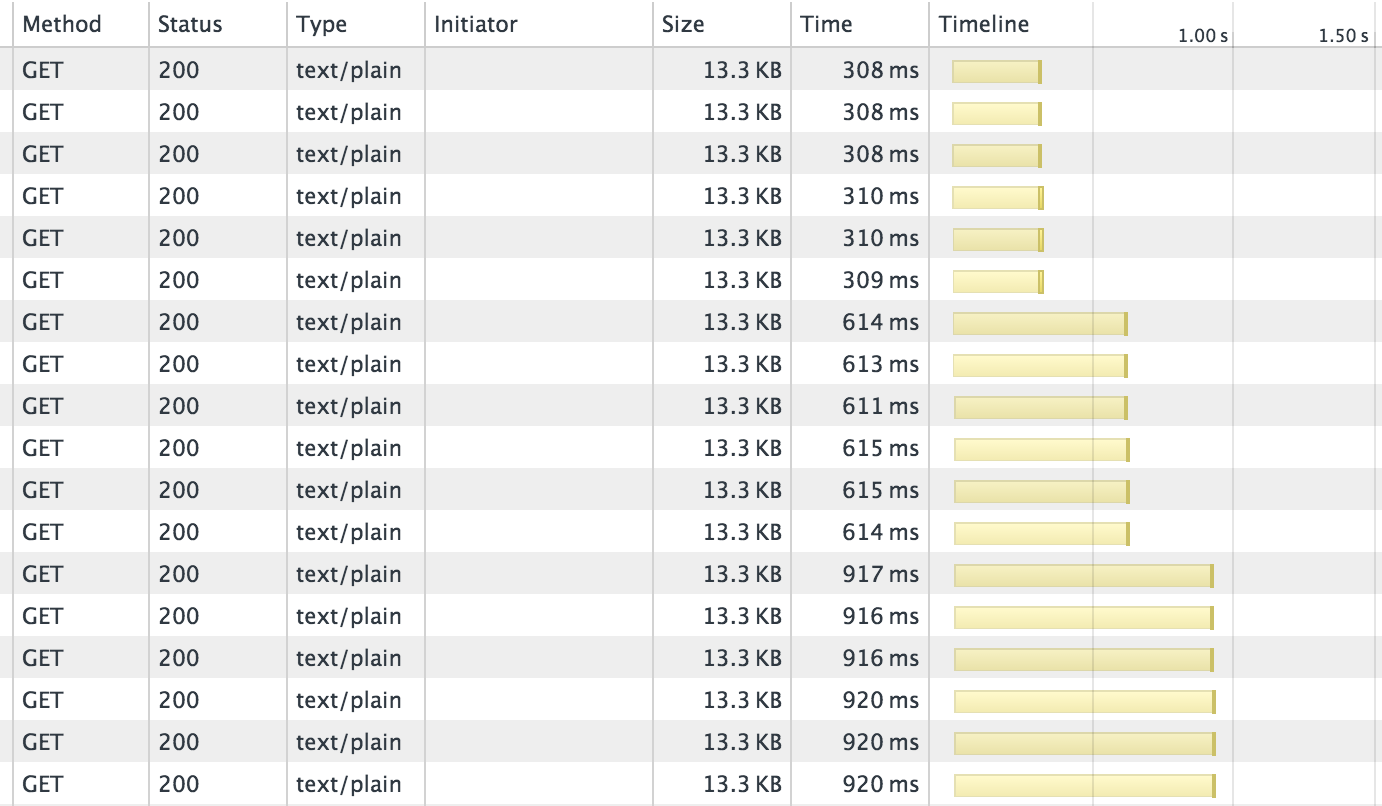
\includegraphics[width=0.9\textwidth]{images/chrome_latency_limit.png}
    \end{center}
  \caption{Chrome developer tools showing how the six TCP connection limit becomes a bottle neck on a connection with ~300 ms of latency.}
  \label{fig:tcp_bottleneck}
\end{figure}

We can calculate the total amount of delay caused by latency in our example with the following formula:

\begin{equation}
\mbox{total latency} = \mbox{number of thumbnails} * \frac{\mbox{latency per request}}{\mbox{number of parallel requests}}
\end{equation}

In our example, we fetch 60 thumbnails on a connection which has a latency of ~300 ms to the server. Our browser (Google Chrome) can handle six parallel TCP connections which gives us the following result:

\begin{equation}
\mbox{total latency} = 60 * \frac{300}{6} \mbox{ ms}= 3,000 \mbox{ ms} = 3 \mbox{ seconds}
\end{equation}

If we instead could concatenate these 60 thumbnail requests into one request, and the response instead would contain all of the thumbnails---then we would only have to pay the latency cost once. This would reduce the total amount of latency by an order of magnitude, from 3,000 ms to 300 ms, since we only have to pay the price for the latency once and not once for every six thumbnails.

As a side-note, it is worth pointing out that increasing the bandwidth of the connection would not resolve this problem as the latency is the only bottleneck in this example.

It is not uncommon for browsers to wait idle for 100--150 ms before spending 5 ms actually downloading an image. This means that latency often accounts for 90--95\% of the total waiting time for HTTP requests\cite{latency}.

\subsection{Chunked responses}
In the previous example where we fetched thumbnails, we often want to display each thumbnail as soon as each individual image has been loaded. This could cause problems now that we are using one concatenated request instead of a separate request for each image. Fortunately we can utilise chunked responses for this.

The HTTP server can utilise \enquote{chunked transfer encoding} in the HTTP responses in order to send the individual thumbnail data in chunks\cite{chunked} to the client. By doing so, images, or any other type of data, can be displayed in the client as soon as each chunk is available, even out of order if necessary. 

This approach, with concatenated requests and chunked responses, has been successfully been implemented at Dropbox on their gallery software implementation\cite{dropbox_chunked}---much in the same fashion as the previous example.

Chunked transfer-coding is the only encoding which HTTP/1.1 clients are required to understand\cite{chunked_required}. This makes it very attractive to use---especially in the use cases where data chunks can be separated in to logical pieces.

\section{Compression}
\label{compression}

All requested data, such as text, can be compressed before it is sent to the client in order to reduce the transfered data size. A common compression algorithm used together with HTTP requests is GNU Zip (Gzip). Gzip works best on text-based files such as HTML, CSS and JavaScript and has an expected compression rate of 60--80\% when used on text-based files\cite[page 237]{HPBN}.

It is worth mentioning that there are scenarios where Gzip compression applied to very small files can increase the total size because of the Gzip dictionary overhead. This problem can be mitigated by defining a minimum file size threshold\cite{google_gzip}.

As an example, arbitrary user data\footnote{\url{https://gist.github.com/AntonFagerberg/32ddde695fb0e2581176}} for 50 users was created and encoded in JSON format. When this data was requested from a server without compression, the total size of the HTTP request payload amounted to 55,205 bytes of data. By applying Gzip compression to the same data, the content length was reduced to 16,563 bytes of data which amounts to a 70\% space saving. 

\begin{equation}
\mbox{Space Saving} = 1 - \frac{\mbox{Compressed size}}{\mbox{Uncompressed size}} = 1 - \frac{16,563}{55,205} \approx 70\%
\end{equation}

An important thing to note about Gzip compression is that only the payload is compressed in HTTP/1.1\cite{header_compression}. This means that the headers, including cookies, are not compressed which would have otherwise been an additional performance gain. This is one of the improvements which have been addressed in the development of HTTP/2\cite[page 222]{HPBN}.

\section{Further reading}
High Performance Browser Networking - What every web developer should know about networking and web performance, Ilya Grigorik, 2013, O'Reilly Media

\begin{quote}
	An essential book about browser networking performance. It covers many aspects around browser networking and the limitations within the HTTP protocols.
\end{quote}

\vspace{5mm}
\noindent High Performance Web Sites - Essential Knowledge for Front-End Engineers, Ilya Grigorik, 2007, O'Reilly Media.

\begin{quote}
	A book about how to build high performing web sites with technologies which also can be applied inside the API gateways.
\end{quote}

\vspace{5mm}
\noindent Even Faster Web Sites - Performance Best Practices for Web Developers, Ilya Grigorik, 2009, O'Reilly Media.

\begin{quote}
	Follow-up book to High performance Web Sites with additional technologies which can be applied inside the API gateways.
\end{quote}

\vspace{5mm}
\noindent Nine Things to Expect from HTTP/2, Mark Nottingham, 2014, mnot's blog

\noindent \url{https://www.mnot.net/blog/2014/01/30/http2_expectations}

\begin{quote}
	A blog post from Mark Nottingham, chair of the IETF HTTP Working Group and a member of W3C TAG, in which he briefly explores nine tings to expect from HTTP/2.
\end{quote}

\chapter{API gateways in theory}
When developing clients for back-end APIs, you often find that the clients needs and the back-end APIs functionality isn't a perfect match. On top of that, different functionality is often required based on whether the client is a mobile application, a desktop application or something entirely different. The way the clients want to use the API can also radically differ based on what kind of product is being developed.

Not being able to optimise the API for each individual clients needs can hurt the clients performance since it has to do a lot of extra work to refit the back-end's model to its own model---but it can also strain the developer whom may have to refit the API for each new client.

Changing the back-end API is often not possible, perhaps especially in an enterprise environment where things might move slowly. The back-end can be a legacy system which is not allowed to changed, it might be impractical to adapt the back-end for different client types without breaking existing clients or the back-end development team might be strained for any other reason. 

One approach to mitigate these problems is by utilising an API gateway as a new software layer between the clients and the back-end APIs. By introducing an API gateway, API-calls can be modified in many different ways when they flow between the client and the back-end API.

\section{What is an API gateway?}
An API gateway works as a layer between the clients and the servers. For an API gateway to be efficient, it has to be able to modify the communication between the clients and the servers, and by doing so, improve the clients and potentially also the servers performance.

The focus in this thesis is to see how the clients can be optimised in terms of performance but also code complexity and developer productivity. Little regard is taken to optimise the server---the goal is however not to put more strain on the server after introducing the API gateway but to keep it on the same level as before.

\begin{figure}[H]
  \centering
    \begin{center}
      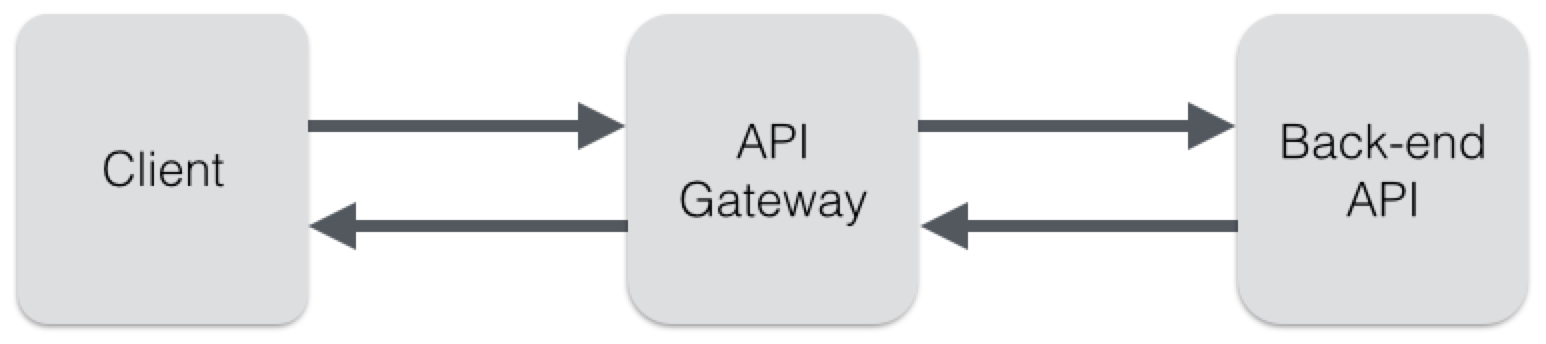
\includegraphics[width=0.9\textwidth]{images/api_gateway.png}
    \end{center}
  \caption{The API gateway is placed as a layer between a client and a back-end API.}
\end{figure}

\section{Differing client needs}
Now, perhaps more than ever, we have a variety of consumer devices such as mobile phones, tablets, desktop computers and other smart devices such as TVs---all of which often consume the same APIs. One can imagine an API which returns a collection of the latest uploaded images to some service. 

Since the screen size is drastically different on a mobile phone compared to a TV, the number of images the client wants to retrieve from the API can be very different. Depending on what type of client is requesting the data, the API gateway can modify the number of returned images.

An approach similar to this has been implemented at Netflix where each client development team write their own \enquote{adaptor} code to fully optimise the underlying API for that clients specific needs\cite{netflix}. This concept works much like how an API gateway works---the main difference being whether the adaptors are actually part of the back-end or in a new software layer.

\section{Multiple resources and requests}
A client often want to perform many requests simultaneously, either to one or multiple back-end APIs. A typical scenarios is when a user loads a single-page web application for the first time and the applications initial state has to be retrieved. Another typical example is when multiple resources, which are connected in some fashion, has to be loaded.

\begin{figure}[H]
  \centering
    \begin{center}
      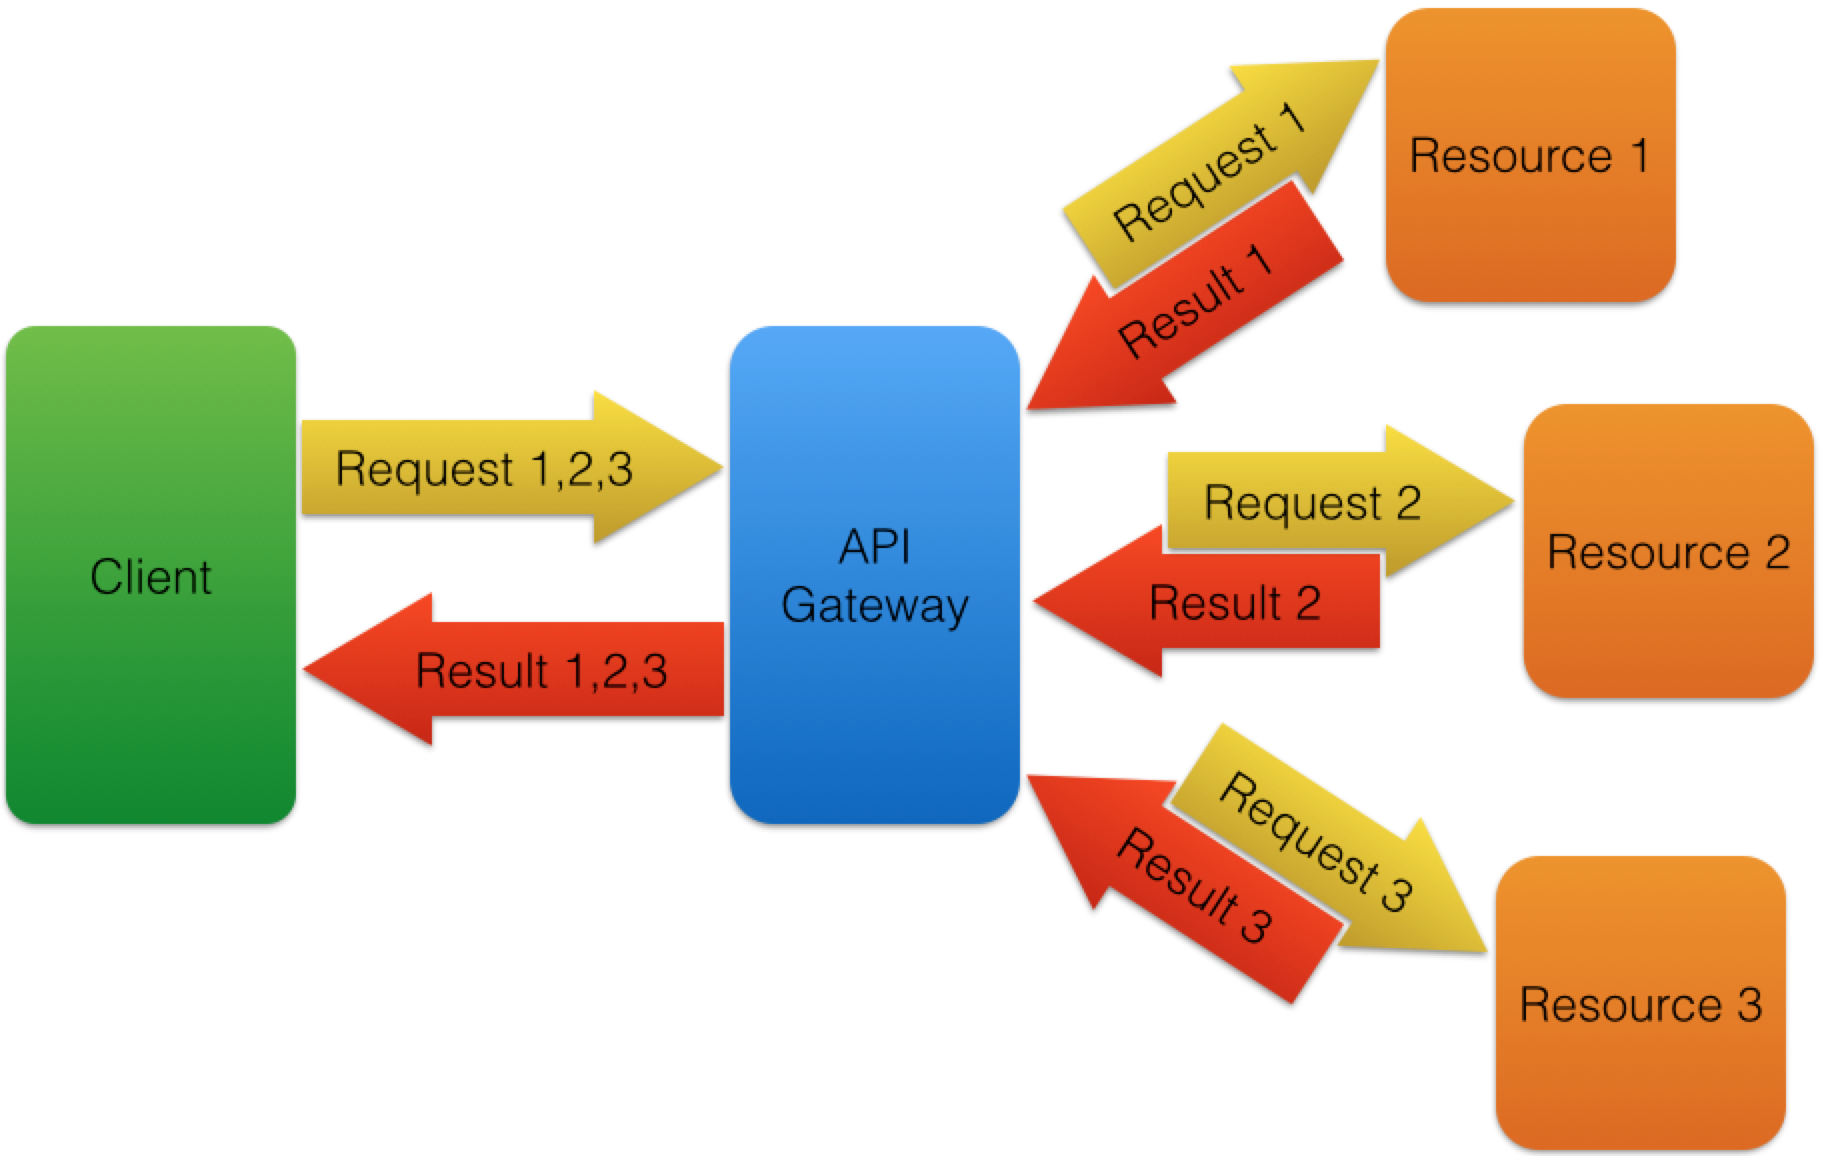
\includegraphics[width=0.9\textwidth]{images/api_gateway_concatenation.png}
    \end{center}
  \caption{The API gateway receives a concatenated request which it distributes to multiple resources, the responses are then concatenated into a single response. The resources can either belong to one or several back-end systems.}
\end{figure}

When working with HTTP requests, there are multiple penalties for executing many small requests compared to one concatenated request. These penalties includes the previously mentioned limit of maximum TCP connections (page \pageref{max_tcp}) and the overhead from http headers (page \pageref{headers}). 

Concatenating many HTTP requests to one request by utilising an API gateway enables us to avoid common problems such as the TCP connection limit and the header overhead. Concatenating requests can be seen directly in many modern API-designs such as the Facebook Graph API\cite{facebook_batch_requests}---but for the APIs which lacks this feature, an API gateway can effectively mitigate these problems.

\section{Duplicate and unnecessary items}
When requesting data from a back-end API, the responses may contain unnecessary data which the client do not need. In a similar fashion, if a client performs several similar requests, it is possible that all the responses contains some amount of duplicate data. By utilising an API gateway, the results from the back-end API can be modified to remove the items which the different clients does not need.

\begin{figure}[H]
  \centering
    \begin{center}
      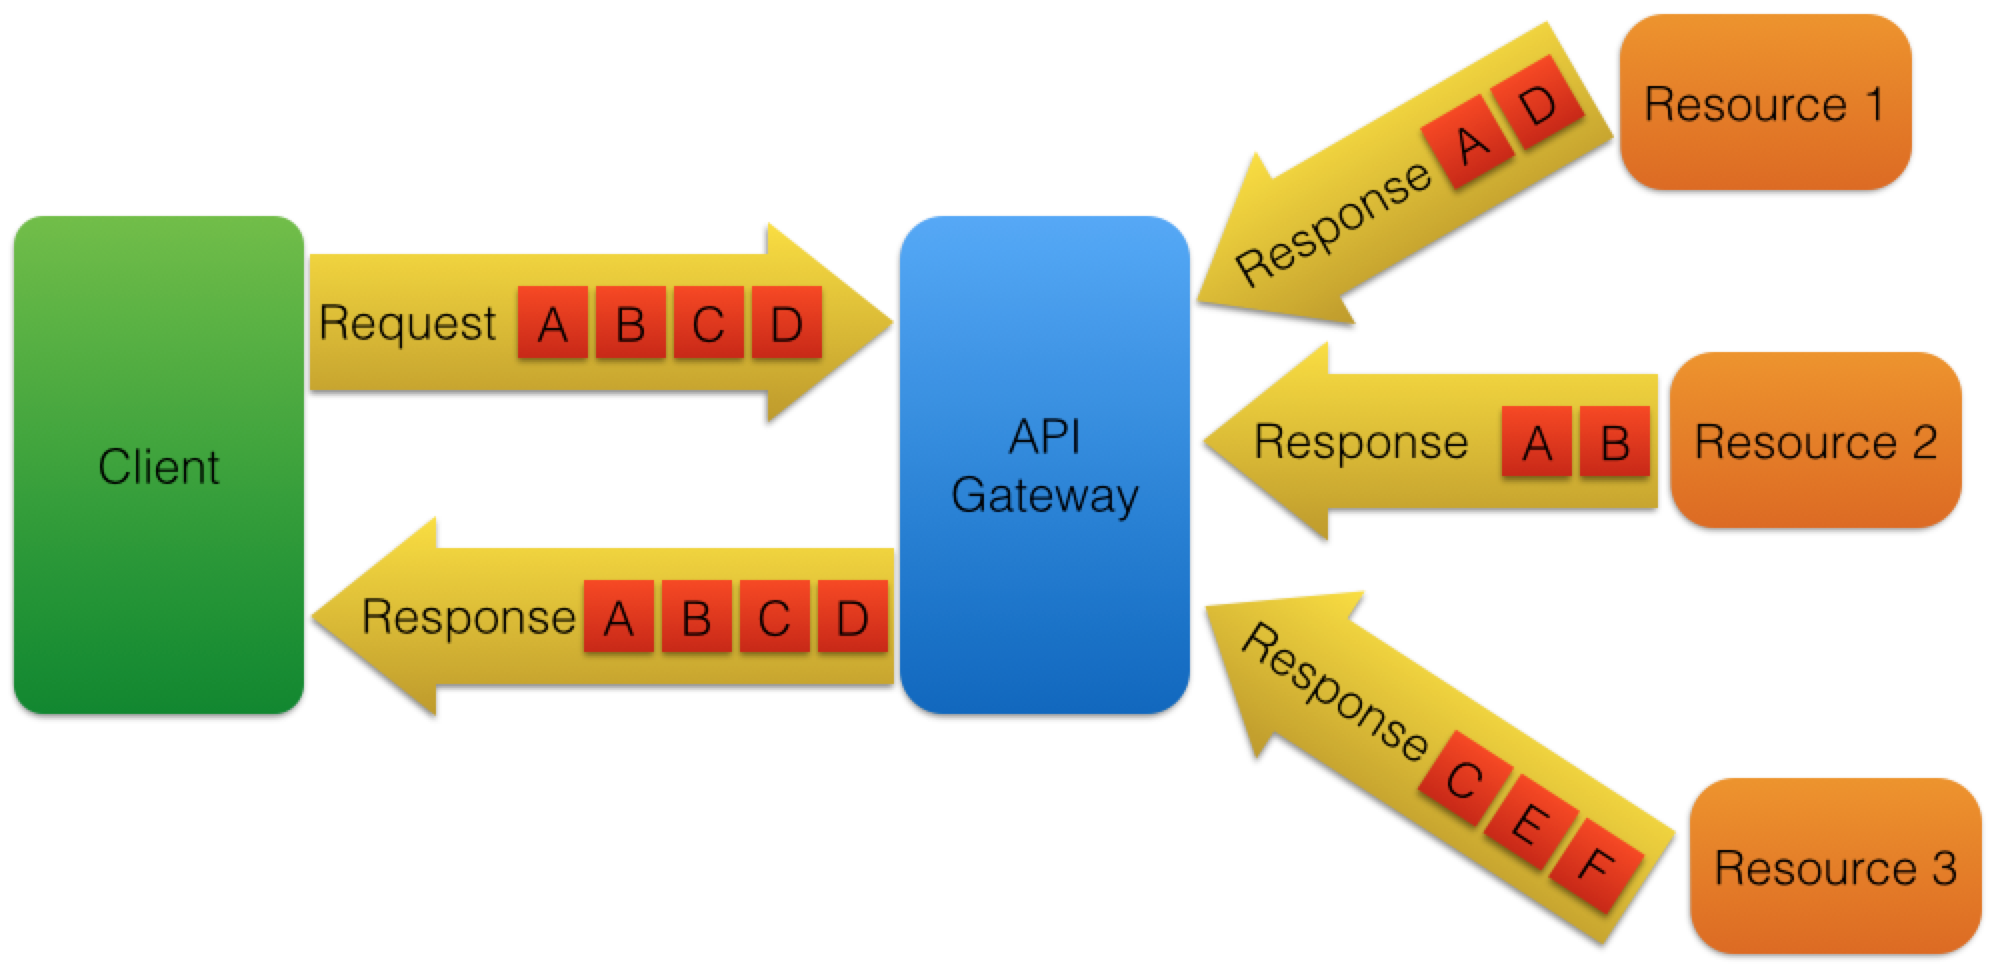
\includegraphics[width=0.9\textwidth]{images/api_gateway_duplicate.png}
    \end{center}
  \caption{The client requests the items A, B, C, D. The API gateway fetches A, D from Resource 1---item A from the Resource 2's response can then be discarded since it's duplicate data. Item E, F from Resource 3 can be discarded since they are not wanted by the client at all. The API gateway can after retrieval respond with just the requested items A, B, C, D.}
\end{figure}

\section{Format transformation}
When working with older legacy systems, the data can be formatted in a way which is not suitable for modern clients. When looking at clients written in JavaScript, many browsers and developers prefer to work with JSON rather than XML since the translation between JavaScript objects to JSON is a 1:1 mapping---more about this on page~\pageref{xml_json}. API gateways can convert the request and response data to a format more appropriate for the requesting client or the responding back-end.

\begin{figure}[H]
  \centering
    \begin{center}
      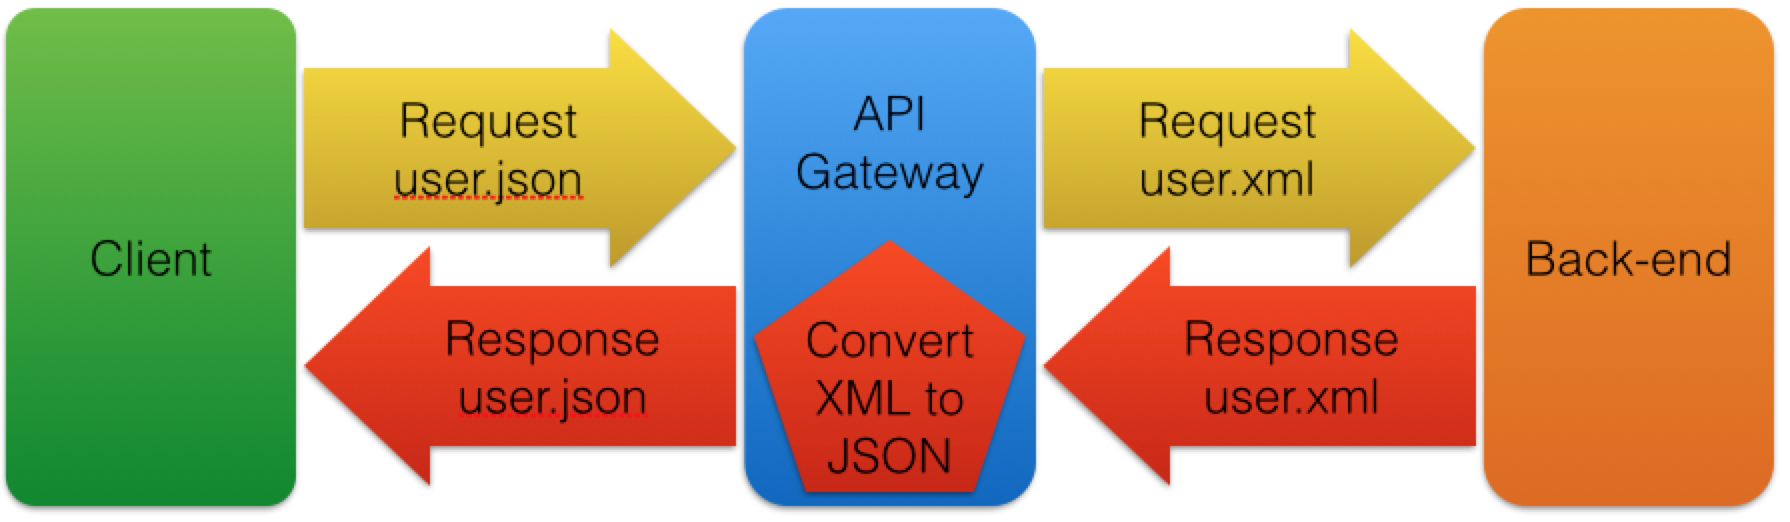
\includegraphics[width=0.9\textwidth]{images/api_gateway_transform.png}
    \end{center}
  \caption{The client requests \enquote{user} in JSON-format. The API gateway fetches \enquote{user} in XML-format from the back-end, converts it to JSON and responds to the client.}
\end{figure}

This approach has the benefit that the conversion code does not have to be rewritten in every client. Rewriting the same conversion code, potentially in a new language or by using a different library, for each client increases the risk of introducing bugs. The reason for this is that different libraries works in different ways even though they solve the same problem, especially when there is no standardised mapping between two formats. Bugs are also introduced as the size of the code base grows when the same task has to be rewritten several times\cite{code_complete}. 

By performing the transformations in the gateway, the processing work is moved away from the clients which can improve its performance as well as reducing the code size and its complexity.

\section{Pure REST and HATEOAS}
If an API follows the strict rules of REST, it utilises the concept of Hypermedia as the Engine of Application State (HATEOAS). Instead of defining and explicitly sharing a collection of end-points which the client can utilise, it requires the client to discover the resources itself by first performing a GET HTTP request to the APIs root URL. The back-end will respond with all the resources available from the root such as \enquote{users}. The client then has to query the \enquote{user's root} to discover which requests can be made in regards to the user's resource---and so forth. 

By forcing the client to discover all resources, the client developer has to do a lot of demanding work in the implementation phase\cite[page 61]{AASG}. This approach also introduces a lot of network requests which increases the traffic significantly.

API gateways can be utilised to transform a \enquote{Pure REST API} with HATEOAS to a simpler API which only follows some of the restrictions put in place by the REST architectural principles. This can significantly lower the amount of traffic between the client and the back-end, which can be a big performance gain, especially in cases such as when the there is a high latency between the client and the back-end---this assuming that the latency between the API gateway and the back-end is low such as when they are placed inside the same LAN.

\begin{figure}[H]
  \centering
    \begin{center}
      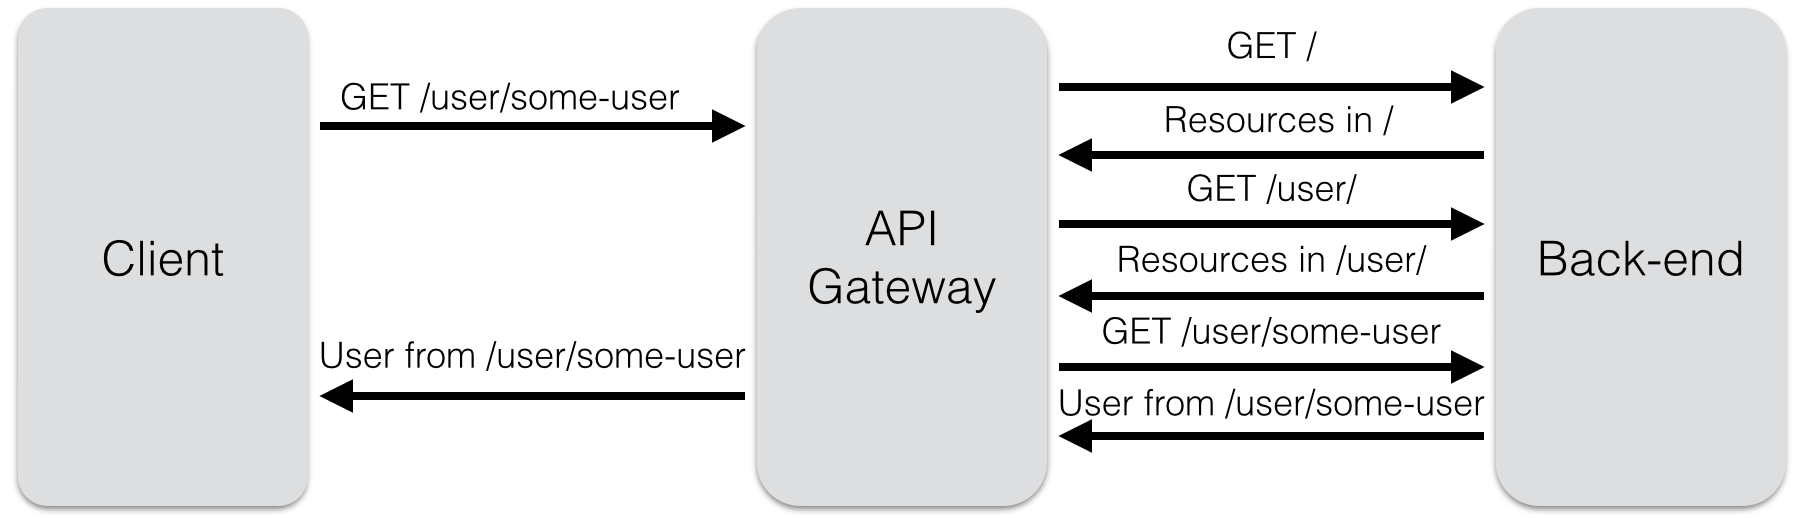
\includegraphics[width=0.9\textwidth]{images/api_gateway_hateoas.png}
    \end{center}
  \caption{The API gateway performs the pure REST HATEOAS communication. At the same, the API gateway exposes a simple end-point which the clients can utilise.}
\end{figure}

\section{Compression}
API gateways can be utilised to compress responses in the cases where no compression is present on the back-end API servers. This can significantly reduce the amount of traffic the client has to receive which increases the performance, especially on mobile devices with low bandwidth. HTTP compression was explored on page \pageref{compression} where it was noted that Gzip has an expected compression level of 60-80\% on text-based media.

\begin{figure}[H]
  \centering
    \begin{center}
      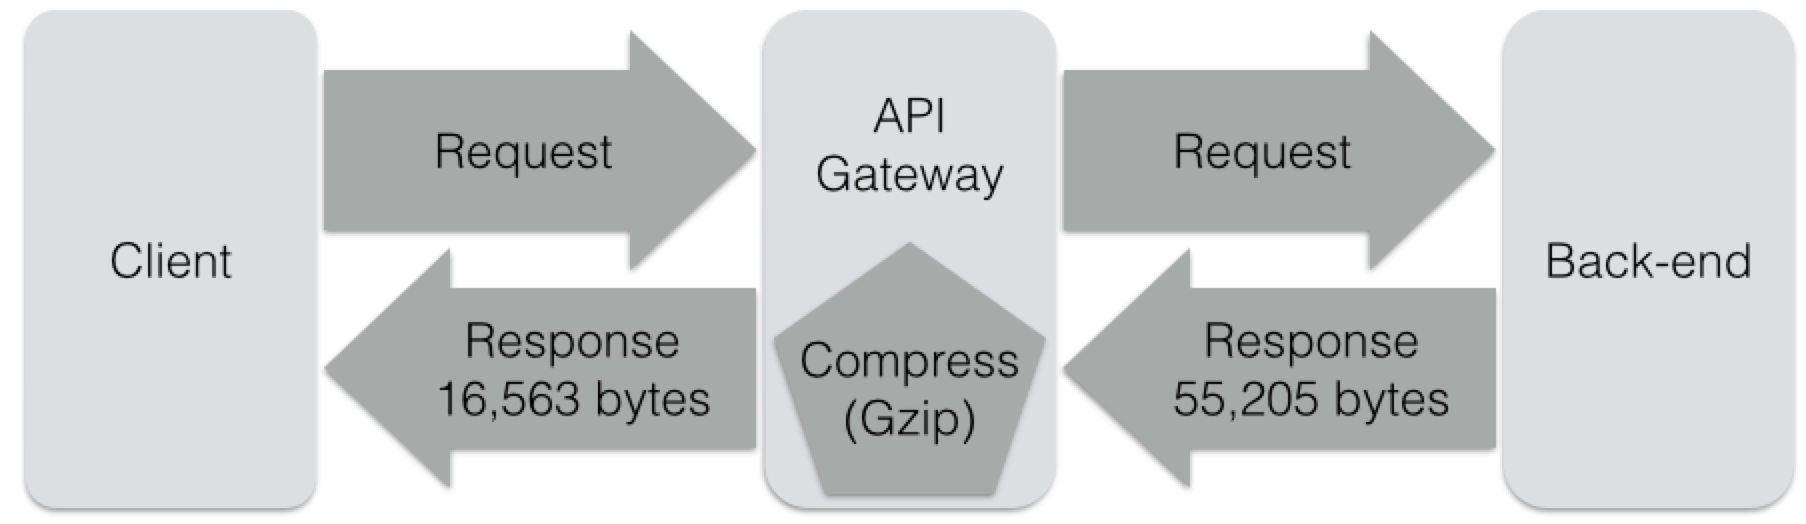
\includegraphics[width=0.9\textwidth]{images/api_gateway_compression.png}
    \end{center}
  \caption{The API gateway compresses the response from the back-end API by utilising the Gzip algorithm. This reduces the response traffic in the client by 70\%. Numbers taken from the example on page~\pageref{compression}.}
\end{figure}

\section{Caching}
\label{caching}
Responses from frequent API calls can be cached using the API gateway to reduce the load on the back-end system\cite[page 107]{AASG}. The cache can have a specified lifetime or be invalidated based on certain events. There are several different caching strategies and many popular third-party systems which the API gateway can utilise---caching is a vast and complex topic in itself and is therefore not explored in further detail here.

\begin{figure}[H]
  \centering
    \begin{center}
      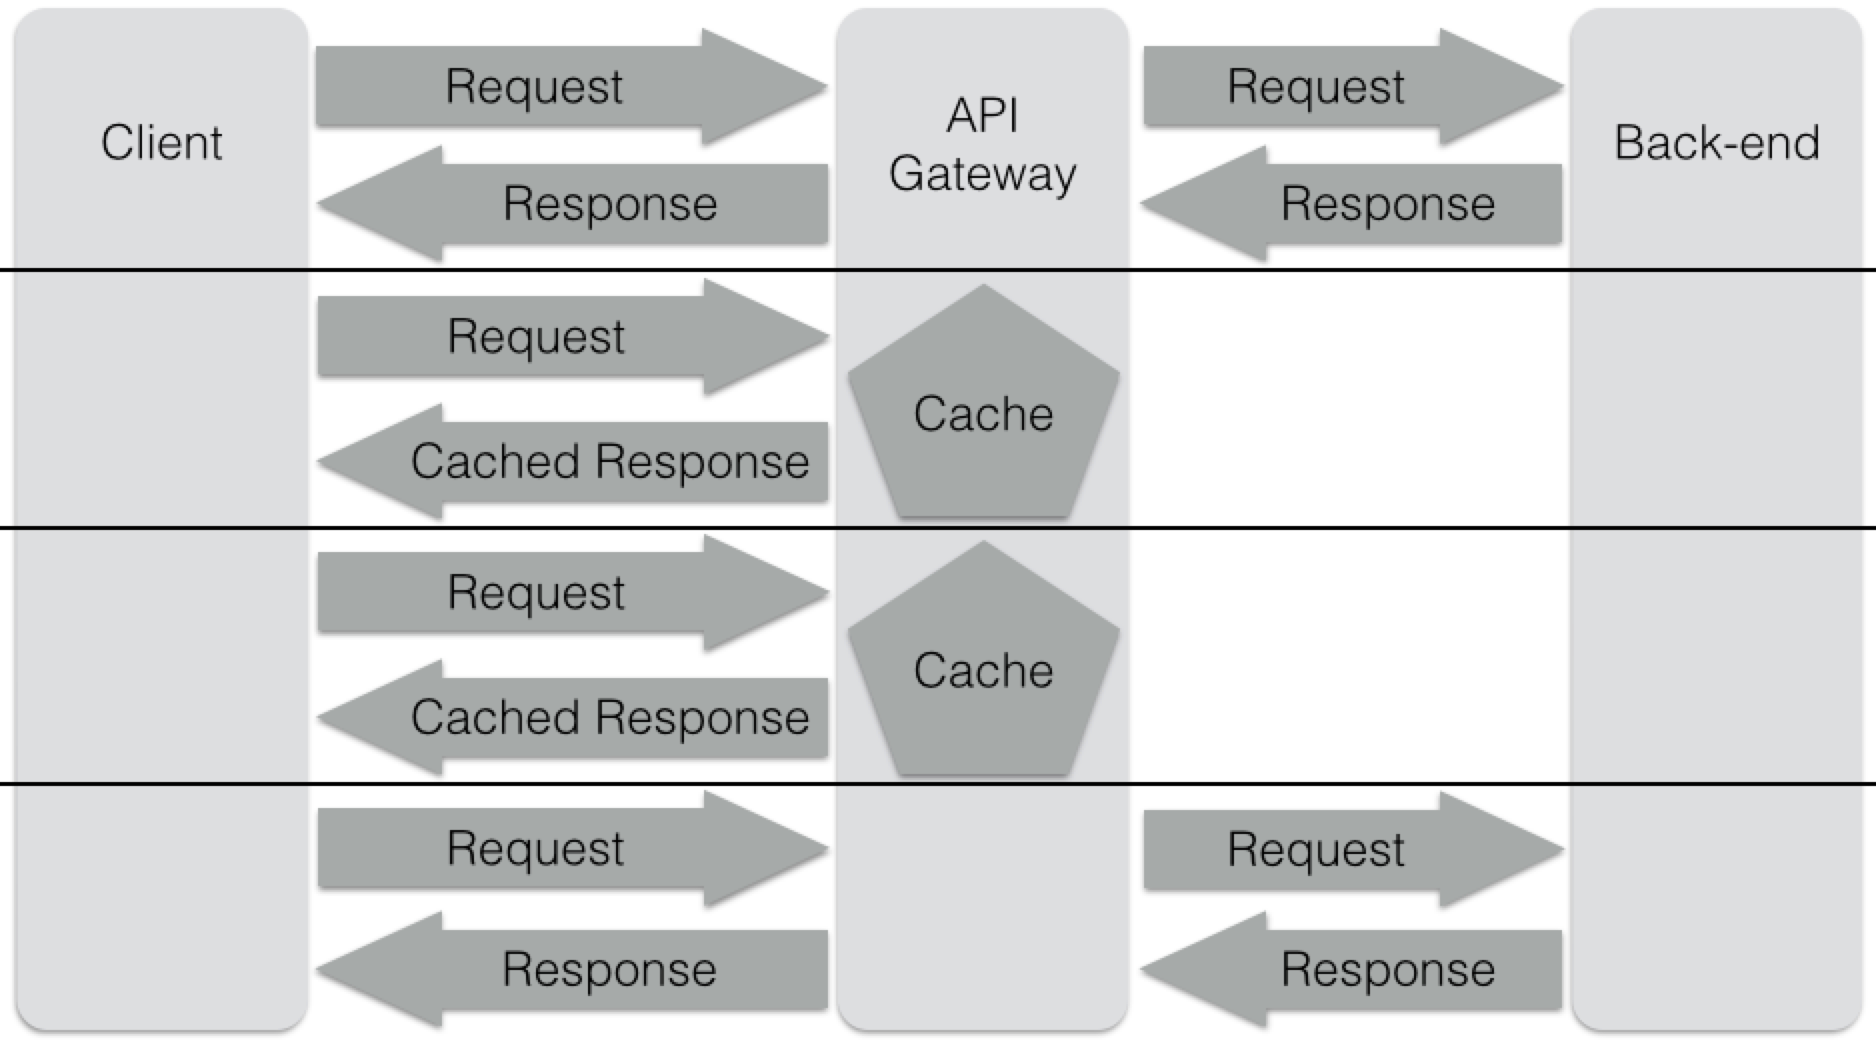
\includegraphics[width=0.9\textwidth]{images/api_gateway_cache.png}
    \end{center}
  \caption{Frequent API calls to the same end-point can be cached in the API gateway to reduce the load on the back-end servers.}
\end{figure}

\section{Decreasing bandwidth and cost}
Cloud providers, such as Amazon\cite{cloud_amazon} and Microsoft\cite{cloud_microsoft}, do not charge for any used bandwidth as long as data is transfered between servers in the same cloud regions. When utilising an API gateway in the cloud, bandwidth and its costs can be reduced by placing the API gateway in the same cloud region as the back-end servers and apply bandwidth saving techniques such as the previously in this chapter mentioned: compression, duplicate \& unnecessary items, pure REST and in some cases even format transformation.

\begin{figure}[H]
  \centering
    \begin{center}
      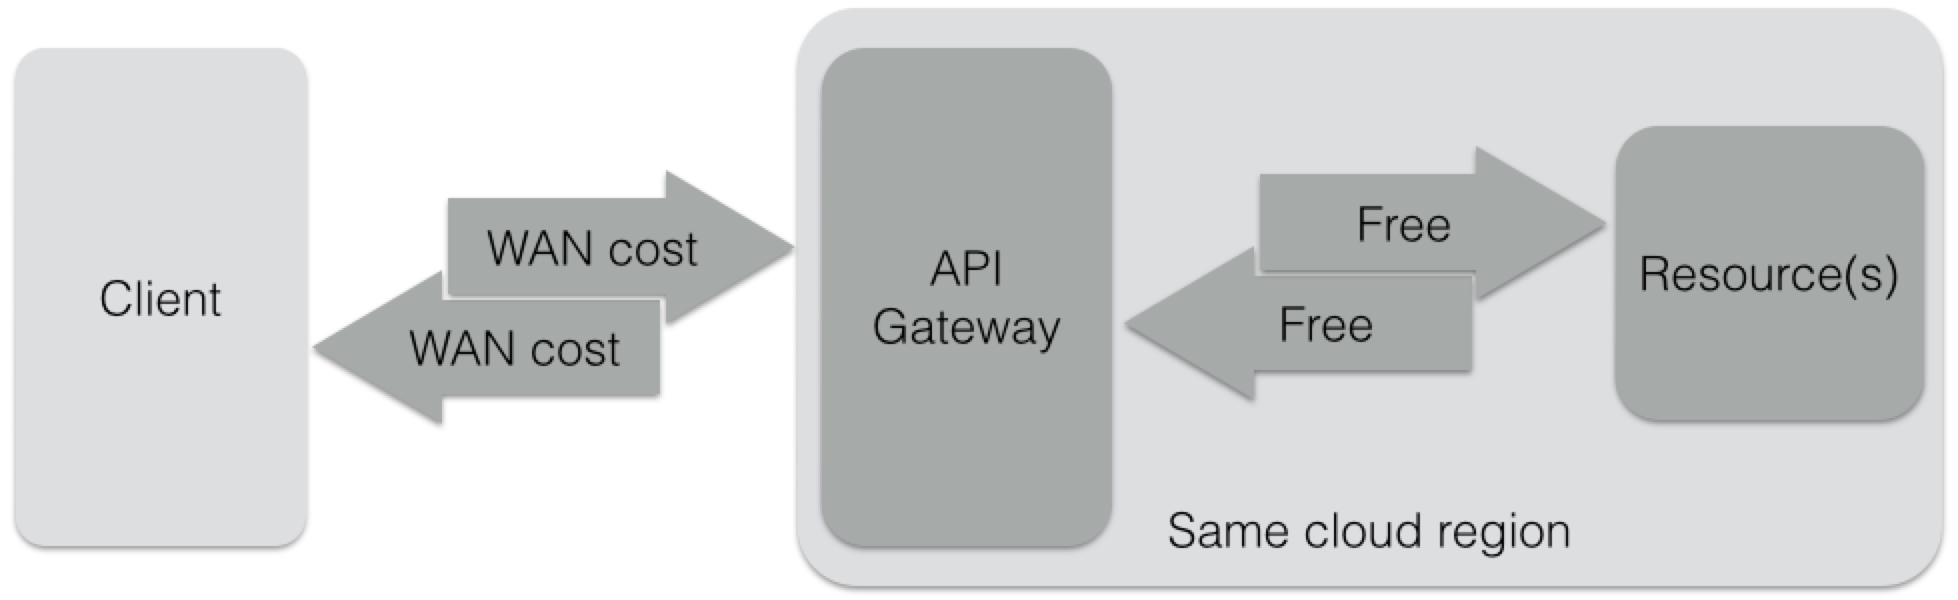
\includegraphics[width=0.9\textwidth]{images/api_gateway_bandwidth.png}
    \end{center}
  \caption{Cloud providers such as Amazon\cite{cloud_amazon} and Microsoft\cite{cloud_microsoft} charges based on whether the traffic is over WAN or in the same cloud region.}
\end{figure}

\section{Secure point of entry for private networks}
Corporations usually uses several internal services with APIs which are protected inside a private network. A VPN, virtual private network, can be utilised to give clients on the outside access to services inside the private network. A VPN can however have the undesired side effect of exposing to much of the private network to the external client machines.

Another approach to solve this is to place an API gateway inside the DMZ of the private network. By doing so, external clients can access the API gateway as a single point of entry for all internal APIs. The API gateway can be configured to only expose a predefined collection of the internal APIs and proxy them to the appropriate external clients.

\begin{figure}[H]
  \centering
    \begin{center}
      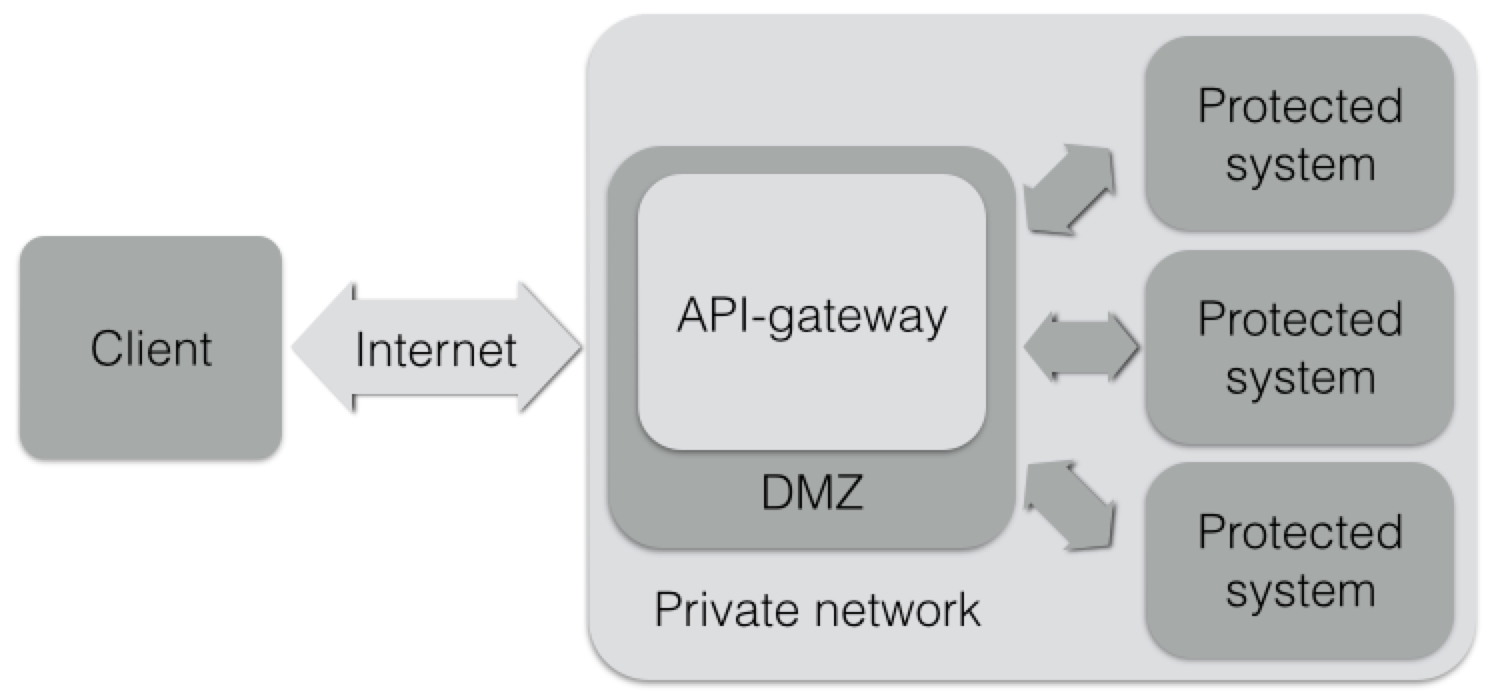
\includegraphics[width=0.9\textwidth]{images/api_gateway_dmz.png}
    \end{center}
  \caption{An API gateway used as a secure way of exposing internal services in a private network to the outside world.}
\end{figure}

\section{Latency}
One important goal of an API gateway is to reduce, or at least not significantly increase, the latency experienced in the communication between the client and the back-end server. Because of this, the placement of the API gateway in a network point of view, is very important. 

The first approach we can look at is to place the gateway on the same LAN as the client. Placing the API gateway on the same machine as the client is rarely possible or practical---it complicates updating the gateway and defeats much its purpose of introducing a new layer between the client and server. 

Placing the API gateway inside the same LAN as the client can be a good solution, for example when used inside a corporations private network. The constraint with this approach is that no outside clients, such as smartphones not connected to the internal network, will be able to avoid the extra latency introduced over WAN---or may not be able to connect to it at all based on the LAN security. This is however an approach which does not introduce double latency---however, it does not decrease it either.

The second approach is to place the API gateway as a separate application in its own cloud or on a LAN separated from the back-end and client. While this may be the only solution for certain hosting setups, this introduces the problem of double latency. Since the TCP-packets has to go through two WAN connections, both of them can introduce a substantial amount of latency which can worsen the response times.

Finally, the third approach is to place the API gateway on the same LAN as the back-end system. This is in many cases the best approach as it avoids the problem regarding double latency while at the same time provides access for outside clients and introduces flexibility in regards to updates. 

The problem with double latency can however arise, and be unavoidable, if the API gateway is communicating with several back-end systems which are placed on different LANs. In such a scenario, several factors have to be considered before deciding which LAN to place the gateway. Such factors include which back-end API has the most traffic, bandwidth costs between LANs, the latency between the different LANs and so forth.

\begin{figure}[H]
  \centering
    \begin{center}
      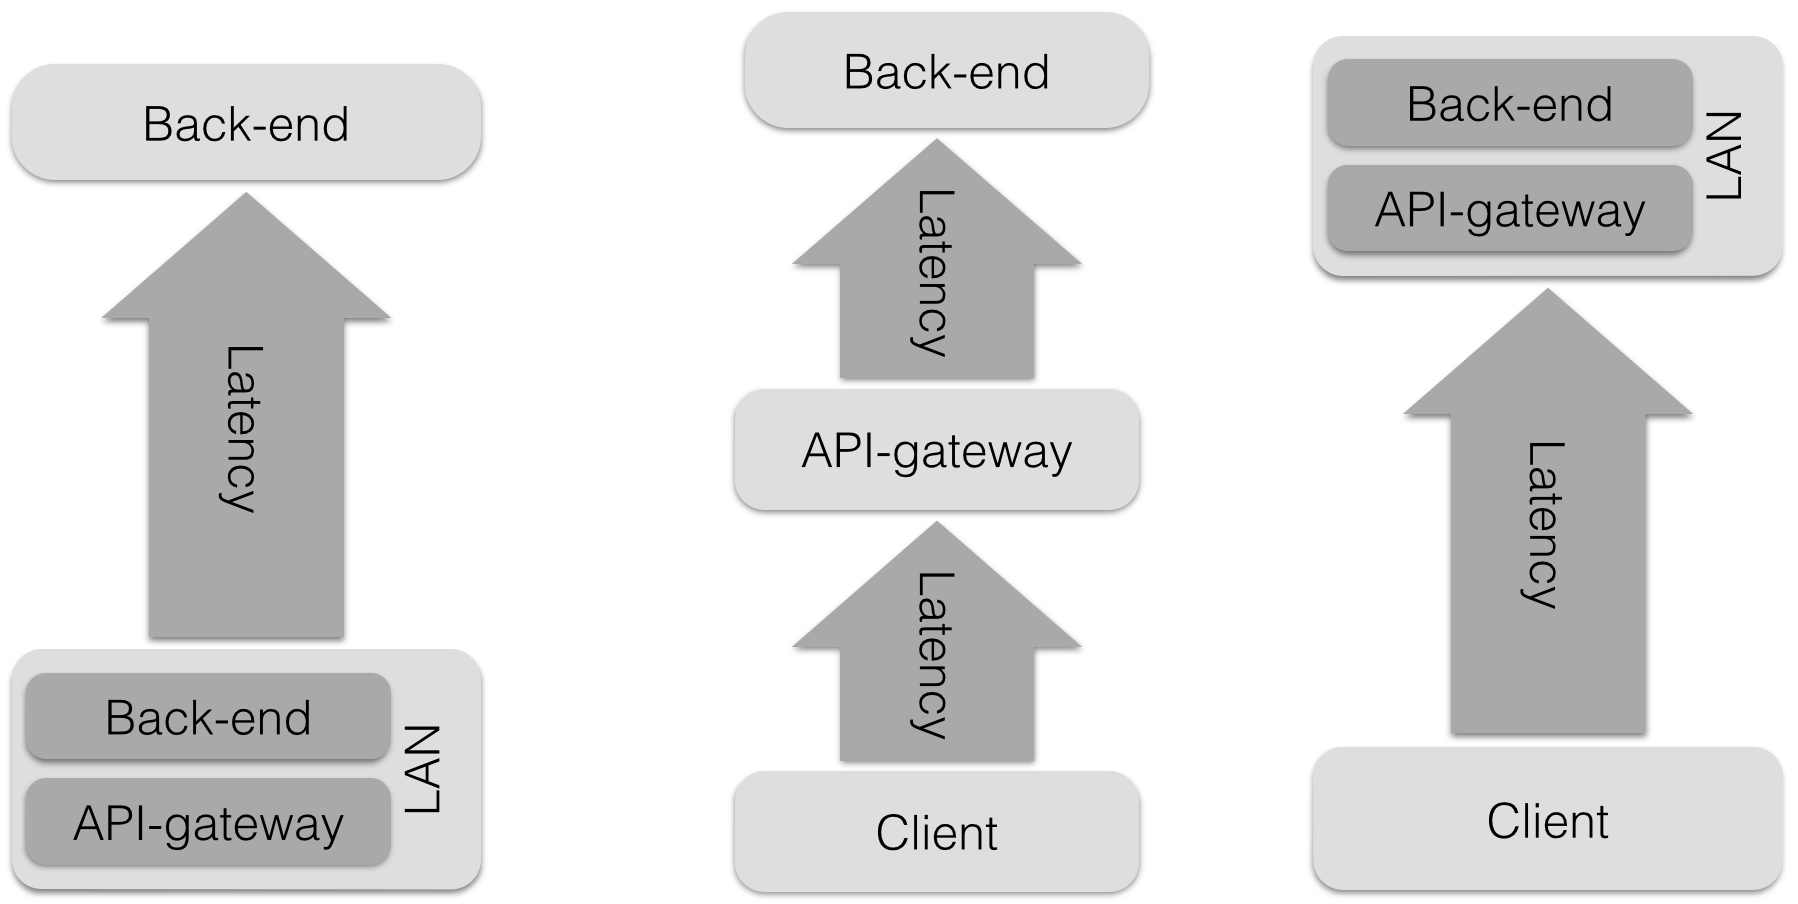
\includegraphics[width=0.9\textwidth]{images/api_gateway_latency.png}
    \end{center}
  \caption{How latency affects the different placement strategies for the API gateway.}
\end{figure}

\section{Error handling}
An API gateway should be able to handle potential errors with different strategies. In the simple scenarios where a single request is proxied and potentially transformed, the API gateway can chose to either resubmit the failing request to the back-end API a number of times, potentially after a small delay, or to simply relay the error to the client.

Deciding what to do in more complex cases where several requests are concatenated or transformed together is much harder. The developer of the API gateway's end-point has to decide if a partial result is relevant for the client or if one failure should invalidate the entire combined result.

Deciding to invalidate the entire result based on one request failure is problematic if the API gateway want to used chunked responses. Ideally, the API gateway want to transmit data to the client as soon as it is available but since chunks can not be retracted, the API gateway either has to wait for all back-end results to arrive before responding or introduce some kind of an error chunk which tells the client to discard the previously sent data.

The API gateway developer always have to make the decision whether to handle much of the error complexity in the API gateway itself or delegate this responsibility to the client. These factors has to be considered on a case to case basis---there is no correct answer.

\section{Security - authentication and authorisation}
\label{sec:security}
API gateway security is, like all security scenarios, a very complex problem. All but the very simplest cases should be solved outside the implementation of the gateway itself in a trusted security solution. What makes an API gateway complex from a security point of view is the fact that one end-point exposed from the API gateway can communicate with several back-end systems, all of which can utilise different authentication and authorisation protocols. Because of this, a single sign-on service provided outside the API gateway itself is a good approach for the more complex API gateways which integrate with several back-end systems.

Any further in-depth discussion regarding this topic is outside the scope of this document and has therefore been excluded intentionally.

\section{Conditional back-ends}
By utilising an API gateway, several different back-ends can be exposed as one single end-point. If we, for example, wanted to provide an API with weather reports from Sweden and Denmark but we have noticed that two different back-end APIs provide better reports for each country---one is better for Denmark and one is better for Sweden. With an API gateway, we can translate the incoming API-calls to the format required by the different back-ends and delegate the call based on certain inputs such as from where the API-call is made.

\section{Rate limiting}
API gateways can make sure we avoid traffic spikes on back-end services by implementing a rate limit of API-calls. This can usually be done in many different ways as seen in Azure\cite{azure_rate_limit} and Apigee\cite{apigee_rate_limit}. Such ways includes a global rate limit, per client rate limit or a per token rate limit. This can also be seen from a business perspective where a certain number of calls are free but a fee has to be paid for subsequent calls.

\section{Support from old API versions}
It happens that API developers makes changes which breaks backward compatibility when moving on to newer improved versions of the API. Fields can be added, renamed or removed. In such scenarios, old clients may be forced to update in order to work with these breaking API changes.

Instead of rewriting many of the already released clients to fit the new API-version, an API gateway can, in some cases, be used to translate the new API format back to the old one. How feasible this is depends on what kind of changes which has been introduced and whether they are destructive or not.

\section{Analytics}
API gateways are in a perfect position to collect data that can be used for analytics. This is because the API gateway is able to monitor all the traffic between the clients and the back-ends. 

\vspace{5mm}

\noindent API gateways can collect a lot of analytic data from HTTP requests and responses such as:
\begin{itemize}
	\item Client technology, the browsers user-agent which is sent with request headers is one way to collect a variety of data. The user-agent normally includes the browsers name and version, rendering engine, computer architecture and operating system.
	\item Request-response time for both the client and each individual back-end API call.
	\item Latency from different back-end APIs.
	\item Geolocation from the HTML 5 geolocation API\cite{html5_geolocation} or by geolocating the requesting IP address.
	\item Errors and failure rates for the back-end servers.
	\item Invalid client requests.
	\item Traffic peak hours.
	\item Suspicious client behaviour such password- or denial of service attacks.
\end{itemize}

\noindent Since performance usually is a top priority in API gateways, the collected data should preferably be delegated, stored and processed using a third-party analytics engine.

\section{Load balancing}
API gateways can be used as load balancers to distribute workloads across multiple back-end systems. This can be achieved by implementing different scheduling algorithms---either by doing a simple round-robin or by implementing a more complex algorithm which takes additional factors into account such as the back-end systems reported load, response time, geolocation and so forth.

\section{Related works}

\subsection{Netflix API}
Netflix has applied a concept similar to API gateways where each client team develops their own end-points adapted to the client's specific need.

\vspace{5mm}

\noindent Optimizing the Netflix API, Ben Christensen, 2013, The Netflix Tech Blog

\noindent \url{http://techblog.netflix.com/2013/01/optimizing-netflix-api.html}

\vspace{5mm}

\noindent The Netflix API Optimization Story, Jeevak Kasarkod, 2013, InfoQ

\noindent \url{http://www.infoq.com/news/2013/02/netflix-api-optimization}


\subsection{Managing API Performance, Apigee}
Apigee does API tool development and has put together a collection of articles with focus on optimising API performance in common scenarios.

\vspace{5mm}

\noindent Managing API Performance, Apigee

\noindent \url{http://apigee.com/docs/content/managing-api-performance}

\chapter{CrocodilePear: API gateway framework}

The framework CrocodilePear was developed in order to better understand and be able to rapidly develop custom API gateways. Existing API gateway technologies, such as Microsoft Azure API Management\cite{azure_api_management}, Apigee Edge\cite{apigee_edge} and IBM API Management\cite{ibm_api_management}, mainly focus on expanding existing APIs from the business point of view with a heavy focus on monetisation, security and BaaS (backend as a service) with drag-and-drop graphical interfaces. 

CrocodilePear's focus, on the other hand, is from a pure technical point of view. The goal is to help developers create their own customised API gateways programatically with a high degree of freedom and a small amount of abstractions which otherwise could limit the use cases. CrocodilePear strives to be very flexible and let the developers create their own custom solutions in any way they see fit.

\section{Technologies: language and libraries}
\subsection{Elixir}
Elixir is a functional language designed for building scalable and maintainable applications which run on the Erlang Virtual Machine. The Erlang VM is known for running low-latency, distributed and fault-tolerant systems while also being successfully used in web development\cite{elixir}. Properties all of which are important when developing a successful API gateway.

Two other important influences for choosing Elixir in this framework is the pipe operator and the asynchronous model achieved by utilising Elixir processes.

\subsection{The pipe operator}
One of the integral parts of Elixir is the pipe operator: \lstinline{|>}. The pipe operator takes the result of the expression left side of the operator and pipes it into the first argument of the right hand side function. People who are accustomed to Unix may see the similarity with the Unix pipe operator: \lstinline{|}.

\vspace{5mm}

\noindent As an example, we can take a look at the following nested and hard to read code:

\begin{figure}[H]
  \centering
\begin{lstlisting}[breaklines=true,frame=single]
Enum.sum(Enum.filter(Enum.map(1..100_000, &(&1 * 3)), odd?))
\end{lstlisting}
  \caption{Elixir code written without the pipe operator.}
  \label{fig:no_pipe}
\end{figure}

\noindent The code from the figure above can be rewritten using the pipe operator which results in a more easily read version:

\begin{figure}[H]
  \centering
\begin{lstlisting}[breaklines=true,frame=single]
1..100_000 |> Stream.map(&(&1 * 3)) |> Stream.filter(odd?) |> Enum.sum
\end{lstlisting}
  \caption{The same code as seen in Figure~\ref{fig:no_pipe} but written with the pipe operator.}
\end{figure}

Another benefit of using the pipe-operator is that it makes you reason about the code in a more structured way. When you read it, you might say something like: \enquote{First I have the range of numbers, then I map over it, then I filter them, then I sum them}---which is then reflected in how the code is written.

The pipe operator is an important part in how CrocodilePear works as it pipes requests to a response, potentially through transformations along the way. For developers who are not accustomed to Elixir, this makes CrocodilePear's syntax look like an easy to read DSL (Domain Specific Language) in which they can expose end-points and pipe requests to the client.

\subsection{Elixir processes}
Processes are Elixir's term for utilising the \enquote{Actors model} as its concurrency model. In Elixir, processes are extremely lightweight (in comparison with operating system processes) which means that it is not uncommon to have thousands of them running simultaneously. Elixir processes run concurrently, isolated from each other and can only communicate by message passing\cite{elixir_processes}.

\subsection{Plug}
Plug is a specification for composable modules in between web applications---but also as connection adapters for different web servers in the Erlang VM\cite{plug}. In CrocodilePear, Plug is utilised for exposing end-points to which the client can send requests, and a as a way for the API gateway to send responses back to the clients over the HTTP protocol.

\subsection{HTTPoison}
Internally, CrocodilePear uses HTTPoison\cite{httpoison}. It is based on on the Erlang project Hackney\cite{hackney}, and it is utilised to send HTTP requests to back-end systems. The HTTPoison library is only used internally and is therefore abstracted away from the framework users to simplify the API gateway development and ensure that it can be removed or replaced in future versions in necessary.

\section{High-level concept}

\subsection{Data structure}
The data structure used in CrocodilePear corresponds to that of an HTTP request. It consists of a numeric HTTP status code, such as 200 for OK\cite{http_status_codes}, headers which is an key-value map and an arbitrary amount of chunks which makes up the actual data payload of the HTTP request/response, in this document called the body (not to be confused with the HTML body-tag).

In addition to this, a meta-data map is available for storing data outside the HTTP-model. This can be utilised to pass intermediate meta-data between requests which are not part of the requests themselves but utilised inside CrocodilePear.

\subsection{Processes: producers and consumers}
The key component in CrocodilePear's asynchronous behaviour is the relationship between producers and consumers. Both consumers and producers are fully asynchronous Elixir processes which communicate by passing messages between each other. When a consumer is ready to receive data from a producer, it sends a message to the producer with its own identity and a status telling the producer that the consumer is ready to receive.

\begin{figure}[H]
  \centering
\begin{lstlisting}[breaklines=true,frame=single]
send(producer, { self, :ready })	
\end{lstlisting}
  \caption{The consumer sends a tuple with status \enquote{ready} and the identity of itself, using the function \lstinline{self()}, to the producer when it is ready to receive data.}
\end{figure}

The identity of the producer is always known to the consumer via an Elixir PID (process identification) which is passed around in the pipeline---the pipeline is explained below. The producer will only produce a response once and will terminate after a consumer has fully consumed the response.

\begin{figure}[H]
  \centering
    \begin{center}
      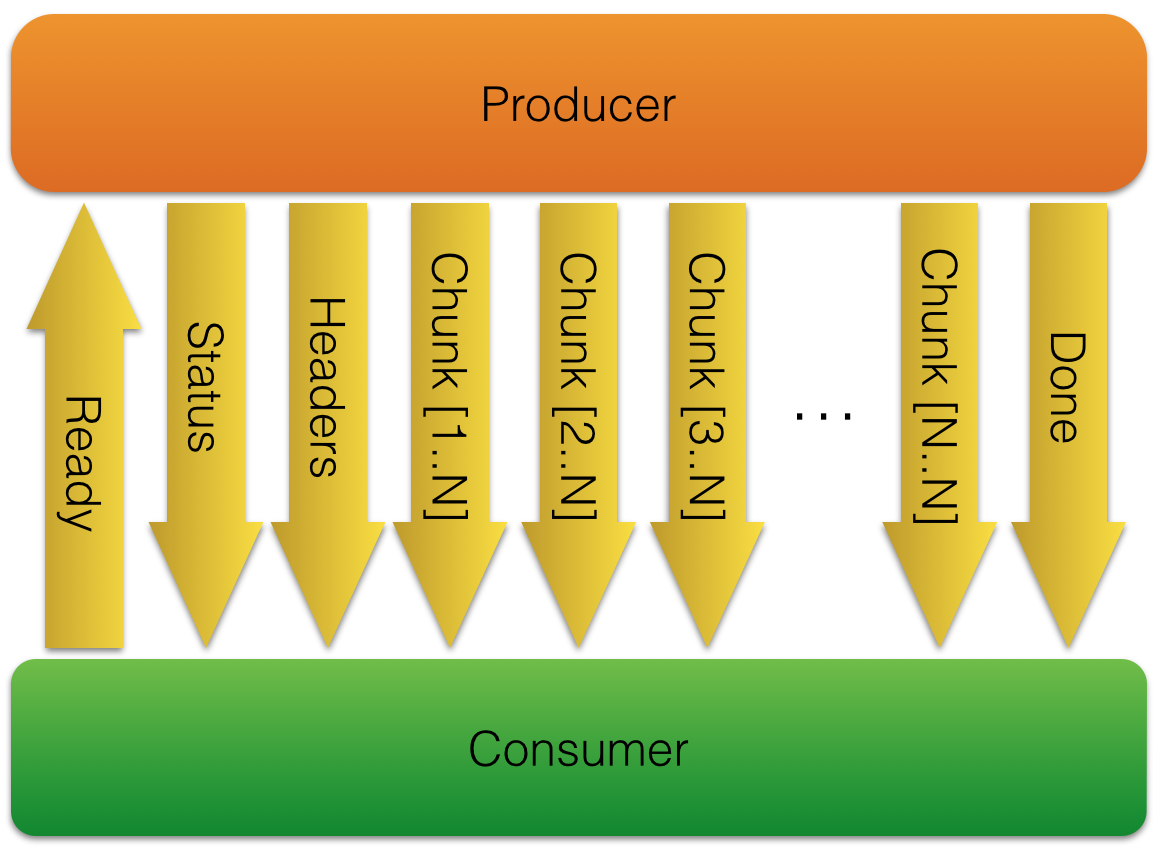
\includegraphics[width=0.9\textwidth]{images/crocpear_producer_consumer.png}
    \end{center}
  \caption{Message passing between a producer and a consumer. Time flows from left to right.}
\end{figure}

After the producer has been notified that a consumer is ready to consume its data, it must first respond with a message containing the HTTP status code, the headers- and the meta data map. After that, the payload chunks must be sent in order. Finally, a \enquote{done} message is sent indicating that the producer will terminate and all chunks has been sent.

All Elixir processes, with the consumers and producers, are abstracted away from the user of the framework. Instead, the end-user only interacts with functions which are applied to all chunks combined on a per request basis. Abstracting away the concurrency model has no performance penalty while it does make the development a whole lot easier since the developer does not have to worry about the message passing. There is however nothing that hinders a developer to work on the lower process level if that for some reason is desired.

\section{Pipeline}
The pipeline is what ties all pieces in CrocodilePear together. The pipeline follows a simple rule: every intermediate function in the pipeline should take a list of producer PIDs as its first argument and return a new list of producer PIDs as its only return value.

The two exceptions are the functions \lstinline{request} and \lstinline{response} which usually are the beginning and the end of each pipeline. It is also possible to mix a CrocodilePear pipeline with a normal function pipeline in Elixir---this is explored further in the examples below.

\subsection{Request}
The \lstinline{request} function in CrocodilePear takes an arbitrary number of URLs as strings or a map structure if more advanced settings is needed such as specifying request headers, the HTTP methods such as GET, POST and so forth. The \lstinline{request} function will always return a list of producer PIDs. Each producer will produce the response from one HTTP request for the specified URL.

\subsection{Response}
The \lstinline{response} function takes a list of producers and turns them in to an actual HTTP response by utilising the provided data structure \lstinline{conn} in the library \lstinline{Plug}. If more than one producer is passed to the \lstinline{response} function, the first responding producer will be consumed first which means that the response order is nondeterministic---if not explicitly defined otherwise. However, the first responding producer will be consumed entirely before any other producer is consumed which guarantees that the chunks from different responses will not be mixed together.

As soon as one of the chunks from a producer has been consumed by the response function, it will respond to the client with it by utilising the chunked HTTP response. CrocodilePear only uses chunked responses which all HTTP/1.1 conforming clients must be able to handle\cite{chunked_required}. Note however that synchronous non-chunking requests, which can be made XMLHttpRequests in JavaScript, will still be able to handle the responses---the only exception is that they will not be able to gain any benefit from the chunking, but there is no downside either.

\subsection{Transformers}
Transformers is a concept used in CrocodilePear to manipulate the response data form a request while it flows through the pipeline without exposing the underlying concurrency model---the Elixir processes and message passing.

The transformer function takes a lambda function (a higher order function) as its only parameter. The lambda function is called with the response data structure as soon as its available as its only parameter which allows transformations to take place.

\begin{figure}[H]
  \centering
\begin{lstlisting}[breaklines=true,frame=single]
blanker = fn(response) ->
  response
  |> Dict.update!(:status, fn(_discarded_status) -> 404 end)
  |> Dict.update!(:headers, fn(_discarded_headers) -> %{} end)
  |> Dict.update!(:body, fn(_discarded_body) -> "" end)
  |> Dict.update!(:meta, fn(_discarded_meta) -> %{} end)
end
\end{lstlisting}
  \caption{The function blanker is a simple lambda function which can be used inside the transformer function. It sets the HTTP status code to 404 and removes all headers, the meta-data and the payload by simply ignoring the received values and providing corresponding empty values instead. The actual data in the status, headers, meta and body are discarded by using an underscore at the start of the variable name in the function call \lstinline{Dict.update!}.}
\end{figure}

\subsection{Timers}
CrocodilePear include timers which can be placed anywhere in the pipeline to benchmark the time it takes to reach the different stages. Timers can be used anonymously or with labels attached to them and they will output the data to the default Elixir logger. The timers also work on the underlying concurrency model which means that every single message in any of the asynchronous processes can be timed individually.

\begin{figure}[H]
  \centering
\begin{lstlisting}[breaklines=true,frame=single]
10:41:57.437 [info]  {1424, 252517, 434960} (Got URL)
10:41:58.187 [info]  {1424, 252518, 187494} [headers] (Executed request) on #PID<0.256.0>
10:41:58.187 [info]  {1424, 252518, 187591} [status] (Executed request) on #PID<0.256.0>
10:41:58.187 [info]  {1424, 252518, 187728} [chunk] (Executed request) on #PID<0.256.0>

[...]

10:41:59.529 [info]  {1424, 252519, 529096} [status] (Added transform function) on #PID<0.431.0>
10:41:59.529 [info]  {1424, 252519, 529177} [headers] (Added transform function) on #PID<0.431.0>
10:41:59.543 [info]  {1424, 252519, 543830} [chunk] (Added transform function) on #PID<0.431.0>
10:41:59.544 [info]  {1424, 252519, 543943} [done] (Added transform function) on #PID<0.431.0>
10:41:59.544 [info]  {1424, 252519, 544106} (Responded to query)
\end{lstlisting}
  \caption{The output from the logger. From left to right: time when message is logged, log level, Erlang timestamp \lstinline{\{MegaSecs, Secs, Microsecs\}}, [message atom] optional message (producer PID if present).}
\end{figure}

\subsection{Concatenate JSON}
The function \lstinline{concatenate_json} takes a list with an arbitrary number of producers, consumes them and returns one new producer. The new producer's chunks will be the responses from the previous consumers, concatenated to a JSON list. Each chunk sent by the new producer will be one item from the JSON list, along with some JSON syntactical data. The order is determined based on which producer starts responding first---just like it is in the \lstinline{response} function.

Each item in the list will be a JSON object which has four keys: status, headers, meta and body (payload). Optionally, if a \enquote{true} value is passed in to the function, each item in the list only contain the \enquote{body} (payload)---the headers, meta and status will be discarded.


\begin{figure}[H]
  \centering
    \begin{center}
      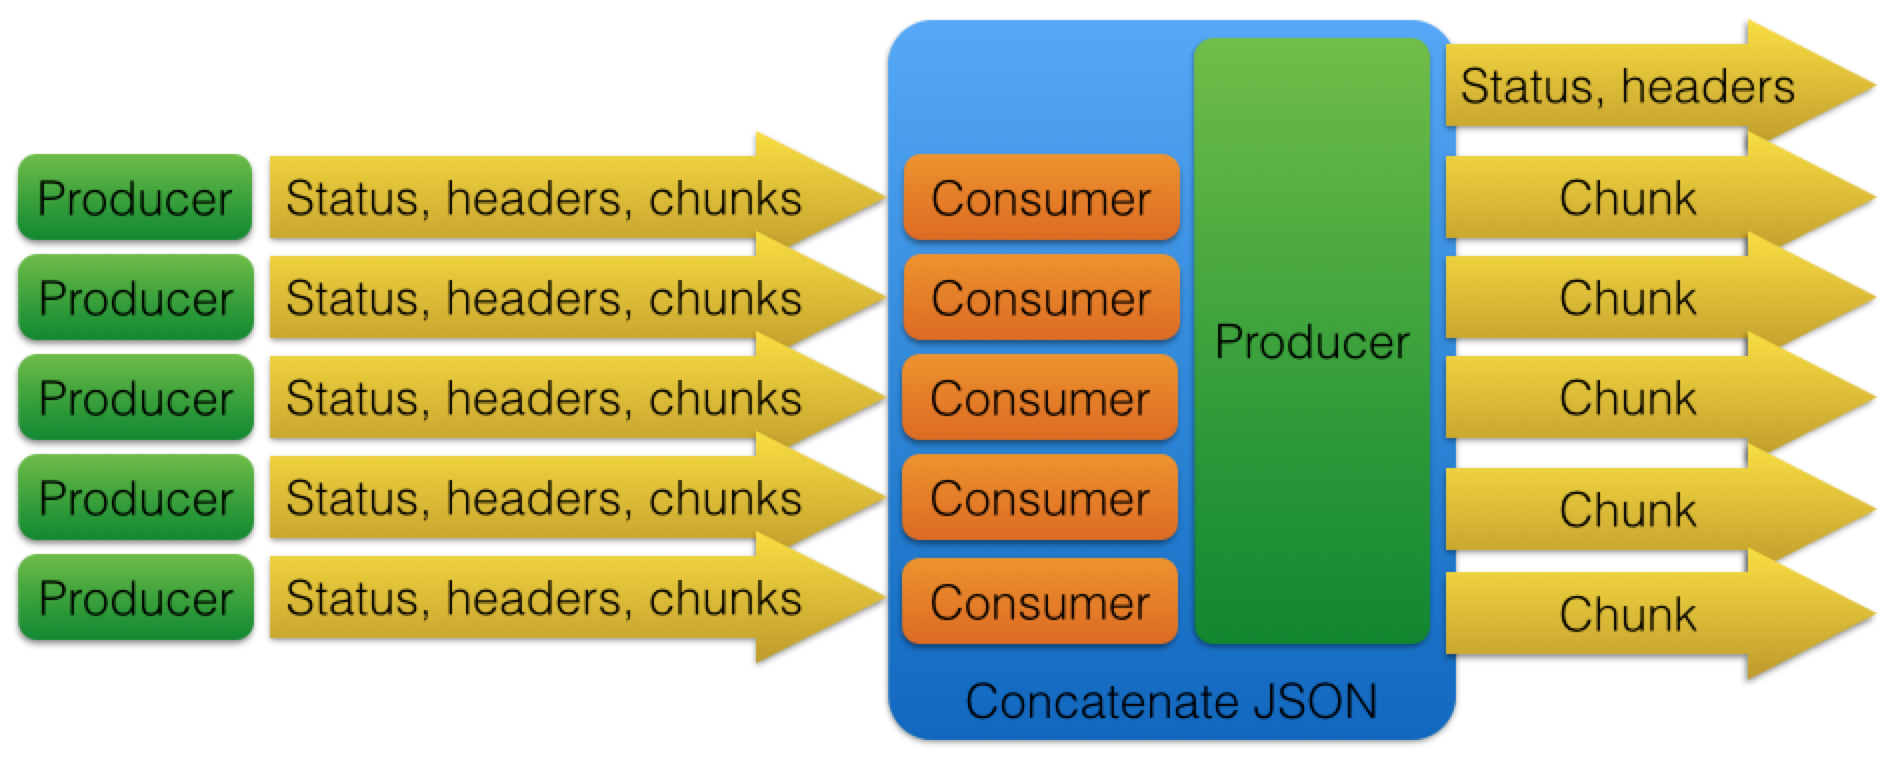
\includegraphics[width=0.9\textwidth]{images/crocpear_concatenate_json.png}
    \end{center}
  \caption{Concatenate JSON creates one internal consumer for each producer. As soon as one consumer has consumed an entire response, the new producer will send that data as a chunk in the appropriate JSON format.}
\end{figure}

Even though \lstinline{concatenate_json} takes an arbitrary number of producer PIDs as its argument, it will itself only return one new producer as its result is one JSON list object.

\section{Examples}
\subsection{Request proxying}
A simple proxy is a good introduction to demonstrates how the request / response pipeline can be utilised. In this example, we extract an URL from the query string from the connection and pipe it to the \lstinline{request} function which itself is piped into the \lstinline{response} function.

\begin{figure}[H]
  \centering
\begin{lstlisting}[breaklines=true,frame=single]
conn.query_string
|> request
|> response(conn)
\end{lstlisting}
  \caption{A very simple proxy.}
\end{figure}

In a similar fashion, we could take an arbitrary number of requests and proxy all of them into one result. Here we take several URLs from the query string separated by the character \lstinline{|} and pipe all of them in to the \lstinline{request} and \lstinline{response} functions as before. By utilising Elixir's \lstinline{String.split}, a list of strings is created which is then passed into the \lstinline{request} function.

\begin{figure}[H]
  \centering
\begin{lstlisting}[breaklines=true,frame=single]
String.split(conn.query_string, "|")
|> request
|> response(conn)
\end{lstlisting}
  \caption{A simple proxy which works with an arbitrary number of URLs.}
\end{figure}

This pipeline execute all the requests concurrently and start responding, in nondeterministic order, based on which one of the requests is responding first.

\subsection{Concatenate responses to JSON}
The \lstinline{concatenate_json} function can be used to concatenate several requests into one JSON list object. It will also automatically set the \enquote{Content-Type} header to the appropriate format \enquote{application/json}.

\begin{figure}[H]
  \centering
\begin{lstlisting}[breaklines=true,frame=single]
String.split(conn.query_string, "|")
|> request
|> concatenate_json
|> response(conn)
\end{lstlisting}
  \caption{Demonstration of the concatenate\_json function.}
\end{figure}

The response will be one JSON list where each item in the list contains the response's status, headers, meta data and the payload as an individual JSON objects.

\subsection{Transformers}
In this more complex example, we will use all the previously explained techniques along with a \lstinline{transform} function to create a much more powerful end-point. We will go over the code from the Figure~\ref{fig:code_transformer} line by line.

\begin{figure}[H]
  \centering
\begin{lstlisting}[breaklines=true,frame=single]
get "/temperature" do
  uris =
    String.split(conn.query_string, "|")
    |> Enum.map(&("http://api.openweathermap.org/data/2.5/weather?q=#{&1}"))

  temperature_extractor = fn(item) ->
    Dict.update!(item, :body, fn(body) ->
      response_body = Poison.decode!(body)

      Map.put(%{}, response_body["name"], response_body["main"]["temp"])
      |> Poison.encode!
    end)
  end

  uris
  |> request
  |> transform(temperature_extractor)
  |> concatenate_json(true)
  |> response(conn)
end
\end{lstlisting}
  \caption{A complex example with a transformer.}
  \label{fig:code_transformer}
\end{figure}

On line 1, we expose the new end-point \lstinline{/temperature} from the API gateway on which we will listen for incoming GET requests.

On line 2--4, we intercept the city names and country codes, such as \enquote{Lund,SE|Copenhagen,DK}, from the query string which is sent with the connection and then split them in to a list using the separating character: \lstinline{|}. This list is then mapped over which will result in the appropriate URLs to call for the underlying back-end API which we will use in this example.

On line 6--13, we create a new transformer lambda function called \lstinline{temperature_extractor}. When we receive the actual payload data, the body, we will decode it from JSON format to native Elixir data structures by utilising the third-party library Poison\cite{poison}. We will create a new JSON object by extracting the name and temperature as a new key-value pair and encode it using Poison again---the rest of the payload data is discarded. The other response data: status, headers and meta, will be kept intact since our function only updates the data stored within they key \lstinline{:body}.

On line 15--19, we tie everything together by creating a new pipeline. We take the URLs, pipe them into the \lstinline{request} function, pipe the result from the \lstinline{request} function in to the \lstinline{transform} function with our new lambda function \lstinline{temperature_extractor}, pipe the result from \lstinline{transform} in to the \lstinline{concatenate_json} function and finally pipe the result to the \lstinline{response} function which will respond to the client.

In this example, we have used the performance enhancing techniques request/response concatenation, discarding of duplicate and unnecessary data, and provided a simple way for clients to request temperature data from multiple cities in one requests with a tailor made response.

\subsection{Timers}
Timers can be used anywhere in the pipeline to output timed logger information. In this example, we use the pipeline from the previous example and attach labels to all the timer functions in order to be able to separate them in the output.

\begin{figure}[H]
  \centering
\begin{lstlisting}[breaklines=true,frame=single]
uris
|> timer("got URIs")
|> request
|> timer("created requests")
|> transform(temperature_extractor)
|> timer("added transformer")
|> concatenate_json(true)
|> timer("concatenated to JSON")
|> response(conn)
|> timer("started responding")
\end{lstlisting}
  \caption{Utilising timers in the pipeline.}
\end{figure}

\noindent The logger for this pipeline would produce an output similar to:

\begin{figure}[H]
  \centering
\begin{lstlisting}[breaklines=true,frame=single]
10:47:49.795 [info]  {1424, 252869, 793251} (got URIs)
10:47:49.815 [info]  {1424, 252869, 796360} [status] (concatenated to JSON) on #PID<0.311.0>
10:47:49.821 [info]  {1424, 252869, 815637} [headers] (concatenated to JSON) on #PID<0.311.0>
10:47:49.894 [info]  {1424, 252869, 890575} [headers] (created requests) on #PID<0.288.0>
10:47:49.894 [info]  {1424, 252869, 894745} [headers] (created requests) on #PID<0.282.0>
10:47:49.895 [info]  {1424, 252869, 891617} [headers] (created requests) on #PID<0.280.0>
10:47:49.895 [info]  {1424, 252869, 891539} [headers] (created requests) on #PID<0.284.0>
10:47:49.895 [info]  {1424, 252869, 894894} [status] (created requests) on #PID<0.282.0>

[...]

10:47:49.903 [info]  {1424, 252869, 903675} [chunk] (concatenated to JSON) on #PID<0.311.0>
10:47:49.903 [info]  {1424, 252869, 903826} [done] (concatenated to JSON) on #PID<0.311.0>
10:47:49.904 [info]  {1424, 252869, 903948} (started responding)
\end{lstlisting}
  \caption{Example output from using timers in a pipeline.}
\end{figure}

\subsection{Simple authentication}
While security is at large outside the scope of this thesis (see page~\pageref{sec:security}), a small example was created to illustrate how a very simple security mechanism can work within CrocodilePear.

In this example, a username and password is retrieved from the URL---note that this is a not secure and this simplified example should not be used in practice! We validate the credentials using a simple if statement and if the credentials are valid, then we create a new \enquote{HTTP Basic Auth} header with a predefined valid username and password (administrator / administrator) which we will use to authenticate ourselves with to back-end system.

What this illustrates is that we can have different credentials for the API gateway and the back-end APIs. CrocodilePear uses Plug which itself, and with third-party plugins, provides several authentication mechanisms such as sessions, cookies and HTTP basic auth.

\begin{figure}[H]
  \centering
\begin{lstlisting}[breaklines=true,frame=single]
get "/http-basic-auth/:user/:password" do
  headers =
    if (user == "test_user" and password == "test_password") do
      [authorization: "Basic #{Base.encode64("administrator:administrator")}"]
    else
      []
    end
  
  %{url: "https://api-url/", headers: headers}
  |> request
  |> response(conn)
end
\end{lstlisting}
  \caption{Simple authentication example---not to be used in practice.}
\end{figure}

\subsection{Caching}
Response caching can be added to CrocodilePear. There are two places where it makes to most sense to add caching in the pipeline. Either we can substitute the \lstinline{request} function with a new \lstinline{request_cache} function or we can do the caching outside the pipeline. 

\begin{figure}[H]
  \centering
\begin{lstlisting}[breaklines=true,frame=single]
get "/proxy/multi/concat-json/cache" do
  String.split(conn.query_string, "|")
  |> request_cache
  |> concatenate_json
  |> response(conn)
end
\end{lstlisting}
  \caption{Individual requests are cached independently of each other with the substitute function \lstinline{request_cache}.}
\end{figure}

The new substitute function \lstinline{request_cache} can cache the requested URLs independent of each other. This means that if we have 50\% of the requests cached, we only have to perform the remaining 50\% requests. The draw-back with this approach is that only the \enquote{raw} responses from the back-end APIs are cached. This means that if we are doing any kind of transformations inside the pipeline, these will be performed on all results---including cached responses. One has to determine if these computations are negligible or if another caching approach has to be taken.

\begin{figure}[H]
  \centering
\begin{lstlisting}[breaklines=true,frame=single]
get "/proxy/multi/concat-json/cache" do
  cache_key = "some_unique_key"
  
  if (has_cache?(cache_key)) do
    get_cache(cache_key)
    |> response(conn)
  else
    String.split(conn.query_string, "|")
    |> request
    |> concatenate_json
    |> response_cache(conn, cache_key)
  end
end
\end{lstlisting}
  \caption{Pseudo-code illustrating how an entire response can be cached.}
\end{figure}

The second approach is to add the response to the cache right before it is sent to the client. This means that not only is the back-end API requests cached but all the computations and transformations as well. This means that the computations does not have to be executed again which was the case in the previous example. The draw-back with this approach is that the entire response is cached as one entity which means that if an end-point does 100 parallel requests where only one request differs, all requests has to be re-added to the cache for every change.

Both these proof-of-concept approaches are naive and there are many things which has to be considered before implementing a caching solution in a real world product such as how long responses should be cached and whether the client should be able to invalidate a cached item and so forth. 

In addition to this, the cache can also be used as a fail over solution where the cache is only used when a back-end server is down or if a request is failing for any reason such as a network failure. As mentioned in the previous section of caching (page \pageref{caching}), caching is a large and complex subject with many aspects which can not be covered in this thesis.

\section{Related works}
\subsection{Tyk}

Tyk is an open source API gateway written in Go which enables you to control who accesses your API, when they access it and how they access it. It can, like CrocodilePear, transform requests but it uses templates instead of code. This approach can make the end-point development easier with the downside of being less powerful.

\vspace{5mm}

\noindent \url{https://tyk.io/}

\subsection{LoopBack-Gateway}

LoopBack-Gateway is an experimental, minimum viable product, API gateway developed by StrongLoop. It is written in JavaScript using Node.js and focuses on rate limiting, reverse proxying and security.

\vspace{5mm}

\noindent \url{https://github.com/strongloop/loopback-gateway}

\chapter{Cases studies}

Three systems was evaluated in order to find potential usage areas for API gateways in real-world products. The goal was to look the three systems from different view points---when two systems has common problems, then it will only be mentioned in one of the case studies. The reasoning behind this was to highlight the different usage potential for API gateways.

\section{Streamflow}
Streamflow\cite{streamflow} is a system used within municipalities in order to communicate with its citizens and inside organisations to communicate with their customers. It is primarily used to register and track customer cases and works as a central case management hub.

Streamflow exposes a HATEOAS API with JSON-encoded responses. The desktop client for Streamflow was written in Java using Swing---however, a new web-client written using AngularJS is currently under development. The following case study has used the in-development AngularJS client using the existing production API which uses HTTP/1.1.

\subsection{Case lists}
In Streamflow, incoming cases are automatically categorised according to the rules defined by the municipality or organisation. Each category has two folders: \enquote{inbox} and \enquote{my cases}. When clicking on the \enquote{inbox} or \enquote{my cases} for a category, all cases in that folder will be fetched from the server and the results will be displayed in a list.

\subsection{Evaluation}
When viewing the case list, several recursive requests will be executed from the client in order to collect all the required information and to follow the HATEOAS specification (the first steps in the request chain has been omitted):

\begin{enumerate}
	\item Request a list of all cases in the selected category and folder. This will return a list of case-objects which are 0.9~KB per object.
	\item For each case in the list, request the case information. This will return the same case-object once more. The reason for executing this request is to discover the next hypermedia resource called \enquote{general}. The wanted payload, the \enquote{general} resource, is 94~bytes while the total response is 3.5--4~KB. This results in a overhead of roughly 97.5\% unnecessary data for each request.
	\item Request the \enquote{general} resource for each case. From this response, the client wants two fields: a date and a note. If a priority is present, the client also wants the next resource called priorities. The total response is 1.5--2~KB and the wanted data is 130~B resulting in a unwanted overhead of roughly 92.5\% for each request.
	\item If the cases has a defined priority, that priority has to be requested. This response is 293~B and will contain information about all priority levels, usually four levels. Each case only has one priority which results in a 75\% overhead for each request.
\end{enumerate}

\begin{figure}[H]
  \centering
    \begin{center}
      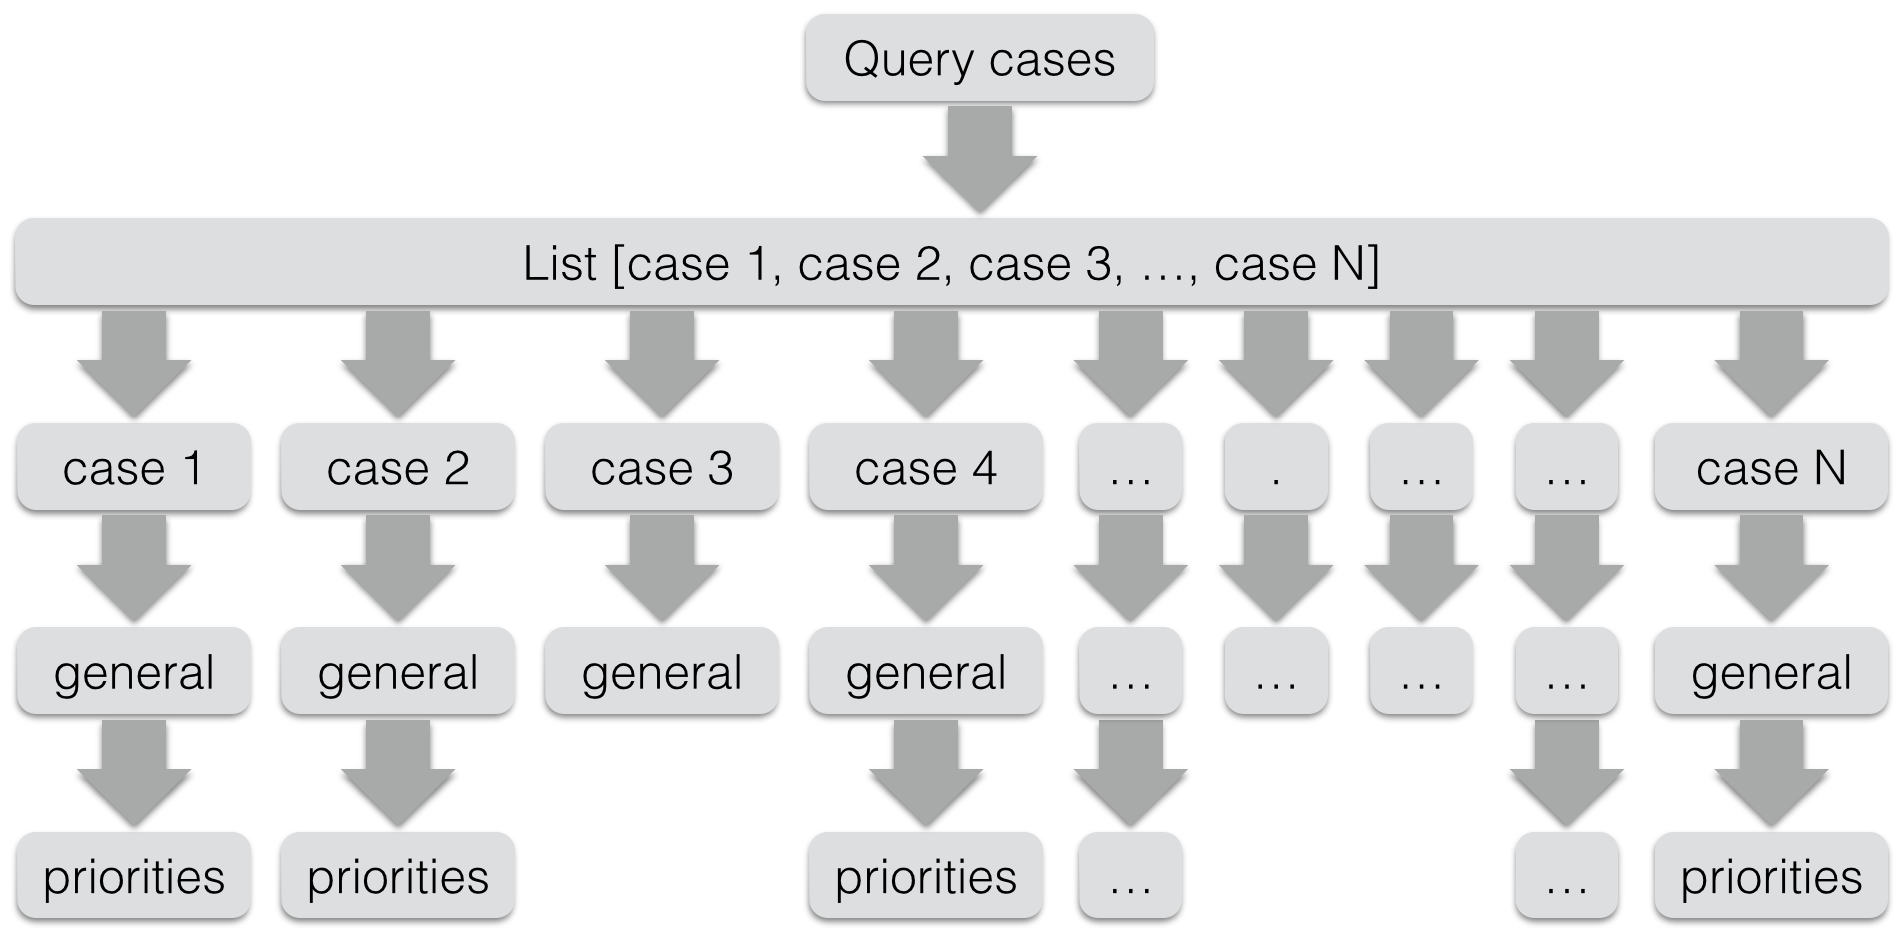
\includegraphics[width=0.9\textwidth]{images/streamflow_cases.png}
    \end{center}
  \caption{How the recursive requests are executed in the Streamflow web client in order to fetch all needed resources and comply with HATEOAS in the REST architectural specification.}
\end{figure}

By placing an API gateway written with CrocodilePear in between the Streamflow web-client and the Streamflow API, all recursive requests can be concatenated, for the client, to one request with a single response. By doing so, a lot of unnecessary data can also be discarded before it is sent to the client. This unnecessary data is duplicate data such as the duplicate case-information, irrelevant data for the client such as HATEOAS discovery information and unneeded data such as unused priorities.

In the test environment, measurements where made on a list which contained 156 cases. For this list, the client had to execute 373 requests---1 request for the list, 156 requests for each case to get the location of the \enquote{general} resource, 156 requests for the \enquote{general} resource for each case, and 60 \enquote{priority} requests for the cases which needed that information. All these request where replaced with one single request to the API gateway which took care of the HATEOAS communication. By doing so, the load time for the client was reduced by 55\%---from 11 seconds to 5 seconds. The total transmitted data was reduced from 1,100~KB to 159~KB---a 86\% decrease of transmitted data.

The Streamflow API does not compress any of the responses. By adding Gzip compression to the payload inside the API gateway before responding to the client, the data could be reduced even more, from 1,100~KB to 9.9~KB, which amounts to a 99\% decrease of transmitted data.

In addition, the client also had to transform certain data types after retrieving them from the server so that it would fit in its internal model. For example, the field \enquote{dueOn} was truncated from \enquote{2015-02-17T23:59:59.000Z} to \enquote{2015-02-17} since the time part was not relevant for the client. By utilising the API gateway, these transformations could be taken care of before replying to the client. This means that no, potentially demanding and error prone, transformations had to be performed on the client---instead the data from the response could be used directly.

\begin{figure}[H]
  \centering
    \begin{center}
      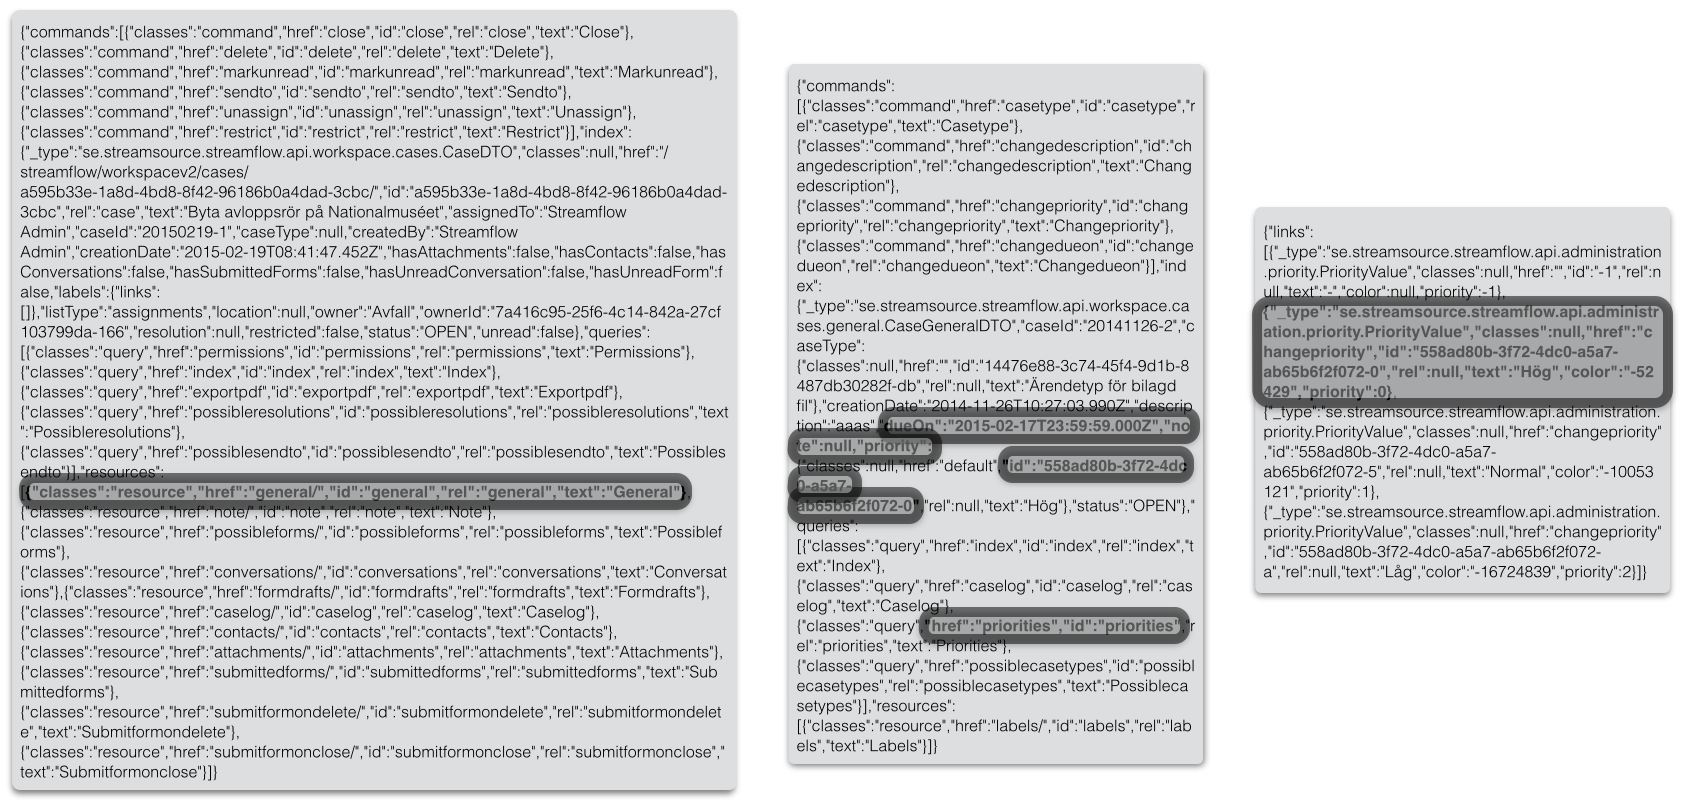
\includegraphics[width=0.9\textwidth]{images/streamflow_response.png}
    \end{center}
  \caption{Illustration of the responses (case, general and priorities) from Streamflow. The actual data needed in the list view is highlighted.}
\end{figure}

In the production environment, a measurement was made to determine the number of cases present in the municipality of Jönköping at a given time of the day. On average, the number of cases in the non-empty inboxes was 19 and the maximum number of cases in one inbox was 296. This means that on average, the number of requests performed, every time an inbox is checked from the client, is roughly 40--60. When the largest inbox is viewed, the number of requests will be somewhere between 600--900---every time it is clicked. This is a substantial performance bottleneck for all clients, especially browsers using HTTP/1.1 considering the TCP max-connection limit and the various textual overheads.

Lastly, it should be noted that the final version of the web-client will most likely be limited to displaying 10--20 cases at a time using pagination. This would reduce the number of requests to 20--60 for any given inbox view. This is however still a substantial amount of HTTP requests to perform every time a user checks an inbox. This approach will neither address the problem that 86\% of the transferred data is unnecessary overhead.

\section{Bank App}
The second system CrocodilePear was evaluated with was a banking app for an undisclosed major bank in Sweden, here after simply called \enquote{Bank App}. Bank App is a mobile app with clients for iOS, Android and Windows Phone. What made the Bank App interesting, from the API gateway point of view, was that it already had a modern and well design API from the start with a design that suited the clients needs. Further on, the clients where written as hybrid apps where common web technologies could be shared among the different platforms and only a small amount of native components had to be changed.

\subsection{Transaction overview}
An essential part of the application is the transaction overview which is where the users can view their balance, orders, fund orders, trades and transactions.

When the transaction overview screen is loaded, the client uses promises (asynchronous computations) to collect and transform the results from the different back-end API end-points. The results are then bound to the scope variable which in turn makes sure that the information is rendered in the view.

\begin{figure}[H]
  \centering
    \begin{center}
      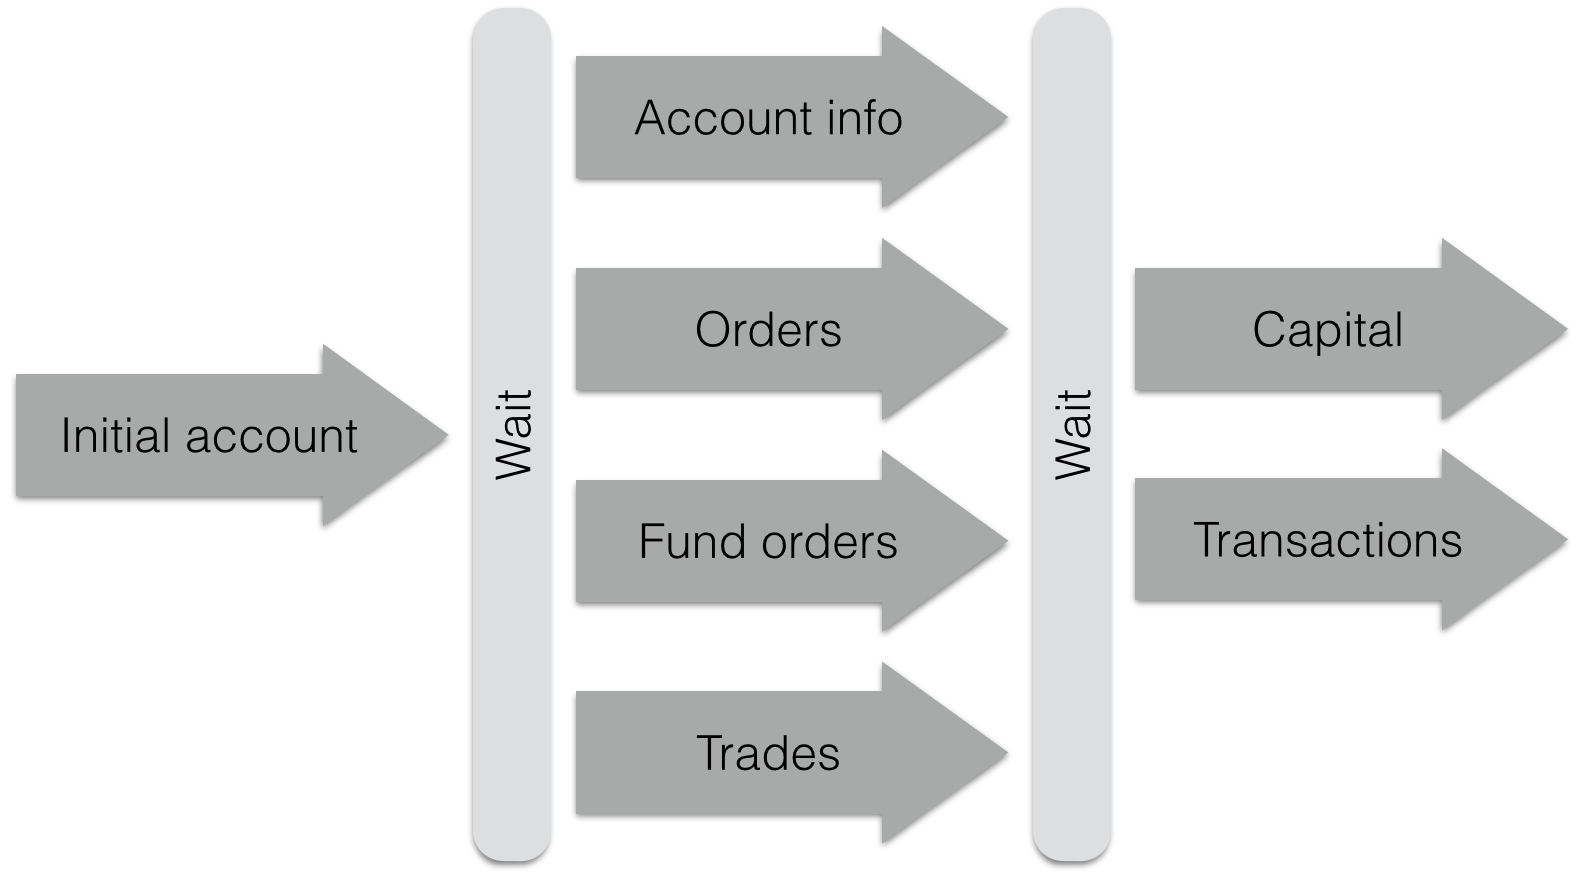
\includegraphics[width=0.9\textwidth]{images/bank_overview.png}
    \end{center}
  \caption{How the asynchronous calls to the API and the transformation works. There are two places where the code waits for previous computations before continuing.}
\end{figure}

To load the required data, the initial account information has to be fetched first. Using that response, the client will then load the account information, orders, fund orders and trades for that account. The client then waits for the four requests to respond, perform some transformations to the data and then merge the it with capital and transactions data so that the fetched information fits the clients internal data model.

\subsection{Evaluation}
All in all, the client requests data from five different API end-points and uses about twice as many functions to fetch and transform these results in the transaction overview. Since the requests are less than six in the transaction overview, it will have no problem with the TCP-connection limit.

The data served from the API only had a small amount of information which the client discarded and so the data transfer before and after the introduction of the gateway was almost identical---about 1 KB less after the introduction of the API gateway.

It is possible that the overhead of unnecessary data can differ from customer to customer. One example of this is the fact that the API sends all of the customer's accounts, including inactive accounts, but the client is only interesting in the active accounts. It is however hard to argue that this amount of overhead is so substantial that it will cause performance issues.

One thing that made the Bank App special is that the different mobile platforms shared a common code base for the overview screen. This meant that iOS, Android and Windows Phone could utilise the same JavaScript code for transforming, filtering and sorting the requested data.

If the Bank App instead was developed by using native code, we would see that the fetching and transforming code had to be rewritten for each platform in a new language. If we draw a parallel to the industry average defect rate, about 1--25 errors per 1000 lines of code\cite{code_complete}, this means that every new client platform introduced to the transaction overview would potentially create 0.1--2.5 new bugs---a number which could be reduced if the code only had to be written once in the API gateway instead.

Perhaps more importantly, by moving the code to the API gateway means that the combined codebase would not just be less error prone but would also be more maintainable. If we, to take one example, wanted to sort the accounts in descending order rather than ascending, we could change this code once in the API gateway and avoid updating every client. 

If this code instead was located in the clients, all of them had to be updated individually, probably by different teams, and submitted to the various app stores for a potentially long review process.

Having different code bases for common tasks in the clients would also increase the risk of introducing discrepancies by mistake despite the goal of having identically working clients on all platforms.

In the end, the code in the client to perform these requests and transform the results amounted to roughly 100 lines of code and the corresponding end-point in the API gateway amounted to roughly the same amount of lines.

It is hard to argue for the inclusion of an API gateway in the current state of this project based on the facts that the Bank App already has a shared cross-platform code base and a well suited API with mostly optimised end-points. One can imagine that the need for an API gateway can increase over time if the API is not moving as fast enough or is as flexible as desired and therefore can not meet the clients needs. It is also a possibility that new clients will be introduced later on, clients move to native code bases instead of hybrid technologies or that they will fork the existing cross-platform code base. However, in the current state of the project, the inclusion of an API gateway will not provide any substantial gain.

\section{Accountant System}

Accountant System is a code name for a system used by a large Swedish accountant firm to help them keep track of important documents, tasks and internal priorities. The client is a single-page web application written in AngularJS which uses an existing legacy back-end API. The back-end API communicates entirely with XML-encoded messages over HTTP---but the client only works with JSON internally. Working with JSON in web applications can be considered very beneficial since JSON and its syntax is a subset of the JavaScript language. JSON support is also included in the ECMAScript standard, which JavaScript implements, since version 5\cite{ecmascript_5}. This enables easy (de)serialisation of JavaScript objects to JSON in all modern browsers.

\subsection{Working with XML in JSON clients}
\label{xml_json}

When it comes to converting XML to JSON, and vice versa, there is no standardised approach which can be applied to make the conversions uniform. Even though the formats do solve some of the same problems in regards to data transmission, the semantics and features are inherently different and it is therefore impossible to create a 1:1 mapping between the two formats.

In an article from XML.com\cite{xml_json} which was published by O'Riley Media, a conversion algorithm was developed to highlight some of the issues regarding this topic. One of the examples started with a very simple XML structure defined in Figure~\ref{fig:xml_structure}.

\begin{figure}[H]
  \centering
    \begin{center}
\begin{lstlisting}[breaklines=true,frame=single]
<e>
  <a>some</a>
  <b>textual</b>
  <a>content</a>
</e>
\end{lstlisting}
    \end{center}
  \caption{Simple XML data structure.}
  \label{fig:xml_structure}
\end{figure}

An algorithm was developed to convert the XML-structure to JSON notation. When this algorithm was tested, the first naive approach to convert the structure from Figure~\ref{fig:xml_structure} to JSON would result in the following invalid JSON structure as seen in Figure~\ref{fig:xml_wrong}.

\begin{figure}[H]
  \centering
    \begin{center}
\begin{lstlisting}[breaklines=true,frame=single]
"e": {
  "a": "some",
  "b": "textual",
  "a": "content"
}
\end{lstlisting}
    \end{center}
  \caption{The first attempt to transform XML to JSON. The result is an invalid JSON data structure because of the duplicate key \enquote{a}.}
  \label{fig:xml_wrong}
\end{figure}

The problem with the JSON structure in Figure~\ref{fig:xml_wrong} is that we can not have \enquote{a} as the key in two places in an associative array---\enquote{a} has to be unique. If we try to solve this by converting the values for the key \enquote{a} to a list instead, then we get a syntactical valid JSON structure as seen in Figure~\ref{fig:json_wrong}.

\begin{figure}[H]
  \centering
    \begin{center}
\begin{lstlisting}[breaklines=true,frame=single]
"e": {
  "a": [ "some", "content" ],
  "b": "textual"
}
\end{lstlisting}
    \end{center}
  \caption{The second approach for transforming XML to JSON. The result is a valid JSON structure but the ordering problem has now been introduced.}
  \label{fig:json_wrong}
\end{figure}

However, another problem has been introduced with this approach which is that the element order is no longer perserved. If we would iterate over the values in the XML from Figure~\ref{fig:xml_structure}, we would end up with \enquote{some, textual, content} but when we iterate over our JSON-structure from Figure~\ref{fig:json_wrong} we would end up with \enquote{some, content, textual} which is not the desired result.

\vspace{5mm}
\noindent Based on this, the following conclusions was made by XML.com:

\begin{quote}

\enquote{A structured XML element can be converted to a reversible JSON structure, if all subelement names occur exactly once, or subelements with identical names are in sequence. A structured XML element can be converted to an irreversible but semantically equivalent JSON structure, if multiple homonymous subelements occur nonsequentially, and element order doesn't matter.} \cite{xml_json}

\end{quote}

Note that the algorithm from XML.com is just one approach to solve some of the problem around XML-JSON conversion---there are many additional issues which makes this conversion very complex. As with many things where there is no 1:1 mapping, different library developers and corporations are developing their own standards to handle the conversion.

To humorously illustrate this problem, a tool was created\cite{jsonx_jsonml} which converted JSON to XML with IBM's JsonX standard and then back to JSON from XML with JsonML's\cite{jsonml} standard. These tools follow their own defined conversion standards with different syntactical data. When these conversions are performed recursively with each output added to the others input, you would expect that the formats would stay the same, switching back and forth between JSON and XML---instead the data structure will grow indefinitely until the browser crashes.

In the end---the point is that converting XML to JSON, and vice versa, is troublesome and since there is no 1:1 mapping, it is handled differently in the variety of libraries used today.

\subsection{Translating XML APIs}
In Accountant System, the XML-JSON conversion was handled in two different ways---one way for requests and one for responses.

\subsubsection{Response}

When working with XML responses from the API, the client utilised a third-party library which converted the XML responses to JSON which then could be used as JavaScript objects in the views, often after some transformations. As in the previous examples, this adds additional complexity to the client which now has to transform the responses before they can be properly handled by the client.

\subsubsection{Request}
More interesting is how the requests are made to the API. When we look at a typical REST end-point which is accessed over HTTP, we first have a HTTP verb such as GET, POST, PUT and DELETE which indicates how the underlying resource should be manipulated. In addition to this, we have an end-point which is we communicate with via a URL. Lastly, we add a payload which either contains the data we want to submit or additional parameters which can make the request more specific than what can be expressed by the URL itself.

In the case of Accountant System, we can look at the simplest scenario which is saving a note. To do this, the client has to send the XML-data seen in Figure~\ref{fig:xml_account_example} to the back-end.

\begin{figure}[H]
  \centering
    \begin{center}
\begin{lstlisting}[breaklines=true,frame=single]
<SaveNotesRequest>
  <Notes>
    <JPTEXT>This is the actual note.</JPTEXT>
  </Notes>
</SaveNotesRequest>
\end{lstlisting}
    \end{center}
  \caption{XML-data used for creating a new note.}
  \label{fig:xml_account_example}
\end{figure}


This XML data has to be sent with a POST HTTP request to a specific URL with ends with \enquote{/note/create}. We can reason about what the purpose of the XML is. From the URL we can deduce where the information should be sent and what information we are sending---a note. We can from the HTTP verb POST see that we want to create a new note and in this case, the URL also contains this information since it ends with \enquote{/create}. The only thing missing to complete this action is the actual payload which is the note content, in this case \enquote{This is the actual note.}.

When working with this API, the XML is entirely redundant from the clients point of view and it does not add any value, but for historical reasons the back-end API can not change. This puts an additional strain and layer of complexity in every new client which interacts with the REST API. Not only do the client have to know about the normal interaction methods such as the URL and HTTP verbs but it also needs to maintain a collection of XML-templates and use a different XML-template for every request it wants to execute. It is also worth pointing out that the the actual note amounted to roughly 1/3 of the total payload data and about 2/3 was structural XML data in the example from Figure~\ref{fig:xml_account_example}.

\begin{figure}[H]
  \centering
    \begin{center}
      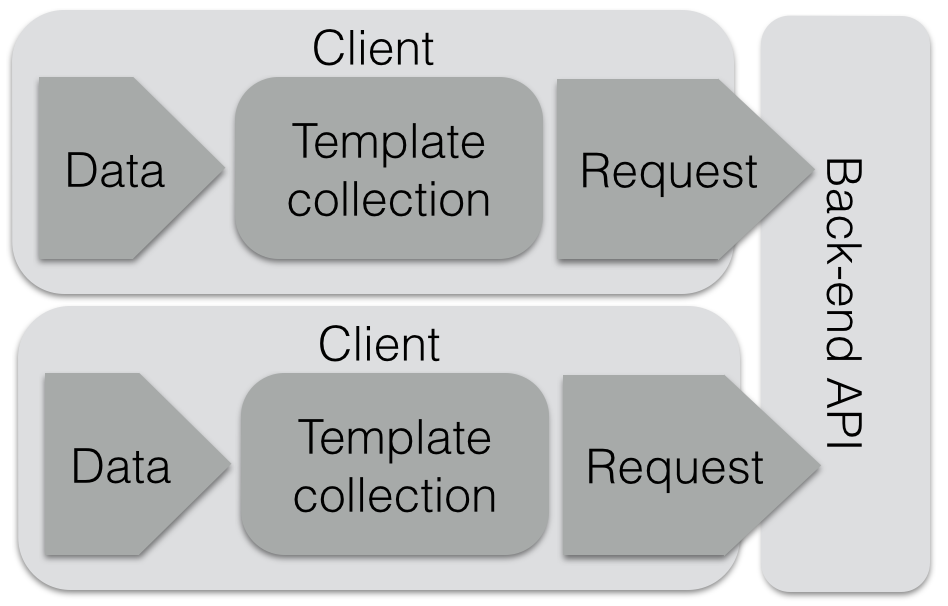
\includegraphics[width=0.9\textwidth]{images/client_templates.png}
    \end{center}
  \caption{Each client has to maintain its own collection of XML-templates in order to make requests to the API.}
\end{figure}

To avoid having to maintain a collection of XML-template in each client, we can introduce an API gateway to do that instead. By introducing an API gateway, we can expose similar end-points which works without any XML in the client. The API gateway will maintain the only collection of XML-templates which it uses for translating the clients API-requests to back-end API requests. This makes the development of clients a lot easier from the API-call point of view but also has the benefit that there is only one, easily maintainable, collection of XML-templates.

\begin{figure}[H]
  \centering
    \begin{center}
      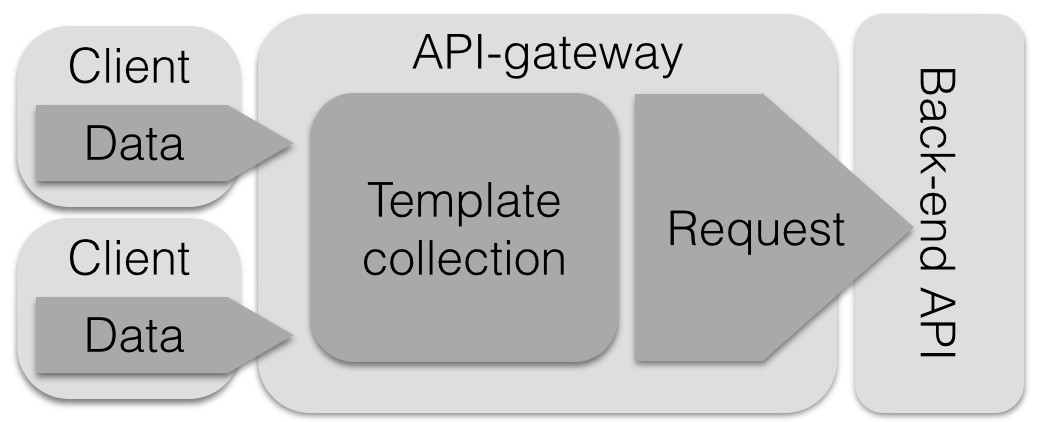
\includegraphics[width=0.9\textwidth]{images/gateway_templates.png}
    \end{center}
  \caption{The API gateway maintains a collection of XML-templates so the client can communicate to the back-end without them.}
\end{figure}

\subsection{Evaluation}

In the case of Accountant Software, we can see a decrease in bandwidth used when dropping the XML-format in the client since XML is a verbose format. A study in 2011 compared the XML-based protocol SOAP (Simple Object Access protocol) with FIX (Financial Information Exchange) and CDR (Common Data Representation) in financial messaging systems and concluded that SOAP had 2--4 times larger messages on average\cite{soap_fix}. It is however hard to draw a fair parallel with that study to this case study.

The biggest gain in utilising an API gateway is likely to be found in developer productivity and code stability. The JSON versus XML is an ongoing debate which has been active for several years. Jeff Barr who is the Chief Evangelist for Amazon Web Services stated in 2003 that 85\% of their API users utilised REST while only 15\% wanted the XML-based SOAP interface\cite{soap_amazon}. The comparison here is not entirely fair either since SOAP is a protocol and not just XML while REST is an architectural style which can utilise XML---and that is the case for Accountant Software.

What we can do is to look at the limitations in XML for Accountant Software in particular. The first thing to note is that all modern browsers has built in support for parsing JSON and there is a natural 1:1 relationship between JavaScript objects encapsulating data and the JSON format. For Accountant Software to work with XML, a third-party library had to be introduced and all API-responses has to be validated to make sure that the JSON-to-XML parsing works in a decent manner as there are pitfalls to watch out for. For clients written in JavaScript, it would be a more natural approach to use an JSON-based API. 

An API gateway can, like the client already do, automatically translate the XML-based responses from the API to JSON. The benefit of placing the translation step in the API gateway is that all clients will translate the XML to JSON in the exactly the same way instead of relying different on local libraries.

\begin{figure}[H]
  \centering
    \begin{center}
      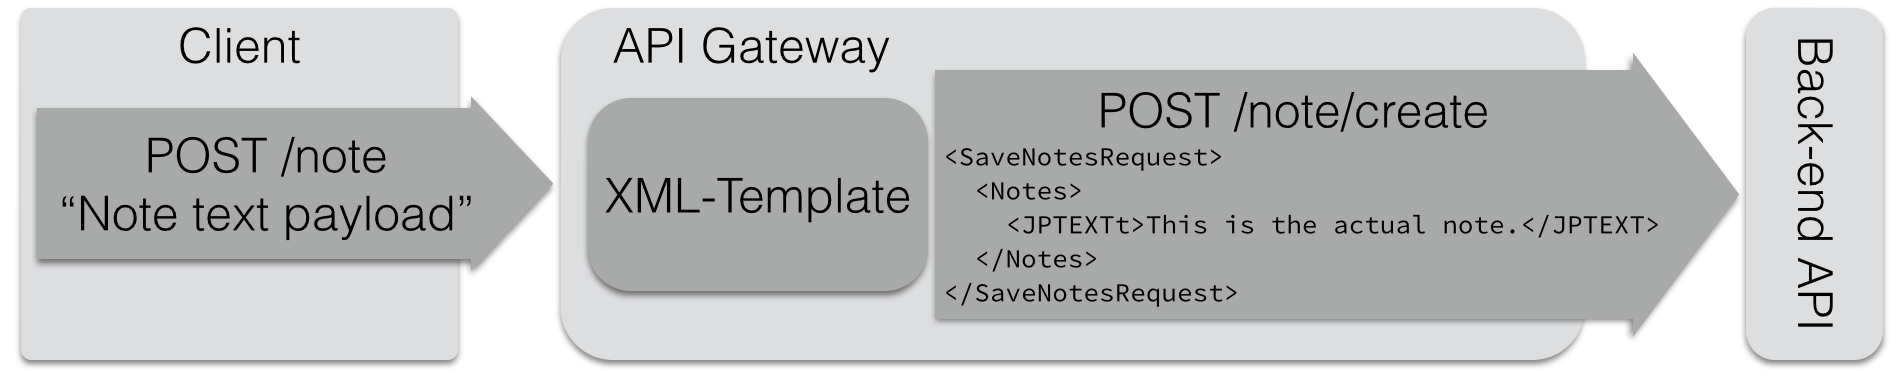
\includegraphics[width=0.9\textwidth]{images/api_gateway_xml.png}
    \end{center}
  \caption{The API gateway exposes a simpler REST interface to the client and converts this to the more complex XML-based interface to the back-end.}
\end{figure}

When looking at the requests to the back-end API, we earlier concluded that the XML in many cases is unnecessary since all information describing data is already present in the URL in combination with the HTTP verb. By moving all XML-templates to the API gateway, all clients can utilise a much simpler API. An additional benefit to this approach is that all XML-templates are gathered in one place in contrast to the current approach where every client has to keep track of their own collection of templates.

\chapter{Conclusions}
As seen in the case studies, the API gateway concept is not a silver bullet and the need for an API gateway varies on a number of factors such as which technology is used in the client and back-end servers, and how well the API can be adapted to the clients needs. We have also seen that API gateways can be used for many different purposes---from network performance to reducing code complexity and increasing developer productivity.

HTTP requests are still very expensive in HTTP/1.1 because of the substantial overhead of headers and cookies. Browsers limits the TCP connection pool to six connections which degrades the performance, especially when the network connection is suffering from a high latency. HTTP/2 will solve many of these issues but a complete switch to HTTP/2 will take many years---the need to change will not only be demanding for the browser- and server developers but all intermediate devices such as proxies has to be upgraded as well. The HTTPbis working group has also announced that HTTP/2 will only work with URLs protected by SSL (HTTPS)\cite{http2_ssl}. This further highlights the need for an optimising API gateway for many years to come. Simple techniques such as request concatenation and data transformations can dramatically increase the performance when looking at the communications between the clients and back-end servers.

From the case studies we have seen that API gateways can be very useful when working with legacy back-end APIs that does not conform to the clients needs. There are many scenarios when the back-ends themselves can not be changed such as when old clients has to be supported or the back-end itself is not actively developed. In such scenarios, API gateways can move the burden away from the clients---by placing the API gateways close to the back-ends, the network costs are negligible. 

The API gateway is not only useful for optimising performance but can also increase developer productivity. By transforming the responses to the format which the clients can handle best, the API gateway can make the client development easier and less error prone while also boasting developer productivity.

API gateways can also be helpful when designing new systems which has to support a variety av clients. This has been seen in the architectural design implemented at Netflix\cite{netflix} which supports many different clients with different needs. In the case of Netflix, the client teams are responsible for developing their own end-points which serves their client a custom tailor-made response. This approach puts the same amount of work on the client and back-end developer teams but lessens the traffic costs, reduces the clients complexity and can increases overall performance.

\section{Future work}

The API gateway concept is very broad and there are many unexplored areas to which the concept can be applied. There are many topics in this thesis which are only briefly touched upon, such security and caching, which could fill an entire thesis of their own in order to be fully explored.

The framework CrocodilePear developed in this thesis used Elixir but there is no doubt that the same functionality could be translated to many other programming languages as well. By migrating the framework to other languages, new challenges and solutions would doubtless appear and shine new light on the topic. 

\cleardoublepage
\phantomsection
\addcontentsline{toc}{chapter}{Bibliography}
\bibliographystyle{unsrt}
\bibliography{anton_msc}

\begin{appendices}
\chapter{Definitions}
\section{JSON}
JSON, JavaScript Object Notation, is a data-interchange text format based on a subset of the JavaScript Programming Language. It is an open standard format which uses human-readable text. JSON is often used as an alternative to XML.

\section{XML}
XML, Extensible Markup Language, is a markup language used for encoding documents. It can be used as an alternative to JSON for data communication but it is also used in other areas and document formats.

\section{REST}
REST, Representational State Transfer, consists of guidelines and best practices for creating scalable web services. The style was developed by W3C Technical Architecture Group (TAG) in parallel with HTTP/1.1. RESTful systems often communicate over HTTP using so called HTTP verbs such as GET, POST, PUT, DELETE to send and retrieve data between clients and servers.

\section{HATEOAS}
HATEOAS, Hypermedia as the Engine of Application State, is a constraint in the REST architecture. The clients enter a REST application through a fixed URL and all future actions are discovered dynamically within resource representations sent from the server.

\section{DMZ}
DMZ, DeMilitarised  Zone, is an isolated subnet located outside the protected LAN where workstations and internal back-end systems are located. It is common that machines, which have to be directly exposed from the internet, are placed inside the DMZ.

\section{SOAP}
SOAP, Simple Object Access protocol, is an XML-based protocol used for data exchange. SOAP is primarily transported using with the underlying protocol HTTP but can also be used with other protocol such as the e-mail protocol SMTP.

\section{Proxy}
A proxy server acts as the intermediary between clients and servers by relaying the data between them.

\section{WAN}
WAN, Wide Area Network, is a network consisting of a large region such as a country or many countries. The internet is considered to be a WAN.

\section{VPN}
VPN, Virtual Private Network, is used to extend a private network, such as in a corporate environment, to an outside public network such as the internet.

\end{appendices}

%\makebibliography{anton_msc}

\end{document}